%%%%%%%%%%%%%%%%%%%%%%%%%%%%%%%%%%%%%%%%%%%%%%%%%%%%%%
\documentclass[12pt, a4paper, italian]{report}
\usepackage{template}  % Assicurati che questo pacchetto esista e non crei conflitti

\usepackage[colorinlistoftodos]{todonotes}
\usepackage{tikz}
\usepackage{tocloft}
\usepackage{adjustbox}
\usepackage{amsmath}
\usepackage[utf8]{inputenc}
\usepackage{listings}
\usepackage{xcolor}

\numberwithin{figure}{chapter}
\numberwithin{table}{chapter}

\usetikzlibrary{shapes.geometric, arrows, positioning, calc}

\lstset{
  language=C++,
  basicstyle=\ttfamily\small\color{black}, % Codice in nero
  keywordstyle=\bfseries,
  commentstyle=\itshape,
  stringstyle=\color{red},
  numberstyle=\tiny\color{gray},
  numbersep=5pt,
  frame=single, % Bordo attorno al codice
  rulecolor=\color{black}, % Colore del bordo
  backgroundcolor=\color{white}, % Sfondo bianco
  tabsize=2,
  breaklines=true,
  breakatwhitespace=false,
  showspaces=false,
  showtabs=false,
  numbers=left,
  showstringspaces=false
}

\tikzstyle{startstop} = [rectangle, rounded corners, minimum width=3cm, minimum height=1cm, text centered, draw=black, fill=red!30]
\tikzstyle{process} = [rectangle, minimum width=3cm, minimum height=1cm, text centered, draw=black, fill=orange!30]
\tikzstyle{decision} = [diamond, aspect=2, minimum width=3cm, minimum height=1cm, text centered, draw=black, fill=green!30]
\tikzstyle{arrow} = [thick,->,>=stealth]

%%%%%%%%%%%%%%%%%%%%%%%%%%%%%%%%%%%%%%%%%%%%%%%%%%%%%%
% packages...
% Package di formato
\usepackage[a4paper]{geometry}		% Formato del foglio
\usepackage[italian]{babel}			% Supporto per l'italiano
\usepackage{lscape}
%\usepackage[a-1b]{pdfx}			% File conforme allo standard PDF-A (obbligatorio per la consegna)

% Package per la grafica
\usepackage{graphicx}				% Funzioni avanzate per le immagini
\usepackage{hologo}					% Bibtex logo with \hologo{BibTeX}
\usepackage{enumitem}

% Citazioni e bibliografia
\usepackage[style=italian]{csquotes}
\usepackage[backend=biber,style=numeric,sorting=none]{biblatex}
\addbibresource{bibliografia.bib}
\usepackage[toc]{appendix}
\usepackage{epigraph}

% Package tipografici
\usepackage{lmodern,textcomp}		% Latin Modern font
\usepackage{amssymb,amsmath,amsthm} % Simboli matematici

% Sistema note a pié di pagina nelle tabelle e nelle figure
\usepackage{footnote}
\makesavenoteenv{tabular}
\makesavenoteenv{table}
\makesavenoteenv{figure}

% Package ipertesto
\usepackage{url}					% Visualizza e rende interattivi gli URL
\usepackage{hyperref}				% Rende interattivi i collegamenti interni

% Path immagini
\graphicspath{ {./images/} }

% Configurazione dei piè di pagina
\usepackage{fancyhdr}  % Per configurare intestazioni e piè di pagina
\pagestyle{fancy}
\fancyhf{}
\fancyfoot[C]{\thepage}  % Piè di pagina centrato con numero di pagina
%%%%%%%%%%%%%%%%%%%%%%%%%%%%%%%%%%%%%%%%%%%%%%%%%%%%%
\setlength {\marginparwidth }{2cm}
\begin{document}

% Frontespizio
\begin{titlepage}
\begin{center}

\includegraphics[width=\textwidth]{Logo.jpg}\\
{\large{\bf Corso di Laurea in Informatica}}
\end{center}
\vspace{12mm}
\begin{center}
{\huge{\bf Black-box per flotte a noleggio: monitoraggio/tracking veicoli, segnalazione allarmi e profilazione guida}}\\
\end{center}
\vspace{12mm}
\begin{flushleft}
{\large{\bf Relatore: Prof. Andrea Trentini}}
{\large{}}\\
\vspace{4mm}
{\large{\bf Correlatore: Dott. Alexjan Carraturo}}
{\large{}}\\
\end{flushleft}
\vspace{12mm}
\begin{flushright}
{\large{\bf Tesi di Laurea di:}}
{\large{Alessandro Belfiore}}\\
{\large{\bf Matr. 975826}}\\
\end{flushright}
\vspace{4mm}
\begin{center}
{\large{\bf Anno Accademico 2023/2024}}
\end{center}
\end{titlepage}


\tableofcontents

\cleardoublepage
\phantomsection
\addcontentsline{toc}{chapter}{Elenco delle figure}
\listoffigures

\cleardoublepage
\phantomsection
\addcontentsline{toc}{chapter}{Elenco delle tabelle}
\listoftables


% o sections (dipende dal documentclass)
\chapter{Introduzione}
Il settore assicurativo è stato uno dei primi a intuire le potenzialità di un tracciamento GPS in grado di registrare gli spostamenti di un determinato automobilista
e di aiutarlo in caso di incidente segnalando ai soccorsi la posizione esatta dell’accaduto, o in caso di furto segnalando alle forze dell’ordine la posizione dell’auto in
tempo reale. Tutto questo è stato possibile grazie all’introduzione della cosiddetta
“scatola nera” o black-box, un piccolo apparecchio da installare sull’auto di un
assicurato, in grado di registrare tutti gli spostamenti di un’automobile, nonchè il
comportamento alla guida del conducente. Può essere utilizzata dalla compagnia
assicuratrice anche per profilare ulteriormente i clienti e offrire quindi delle polizze
ulteriormente personalizzate e fatte su misura per il tipo di utilizzo
\cite{fracassi2012}.
\section{Cos'è una scatola nera?}
La black-box è un dispositivo elettronico utilizzato principalmente per monitorare e registrare vari parametri di funzionamento del veicolo e comportamento del conducente. Sebbene il termine sia spesso associato alle registrazioni di volo degli aerei, nel contesto automobilistico e assicurativo, la scatola nera ha una funzione leggermente diversa ma altrettanto cruciale. Ecco una descrizione dettagliata nei due paragrafi che seguono:

\begin{figure}[h] \centering
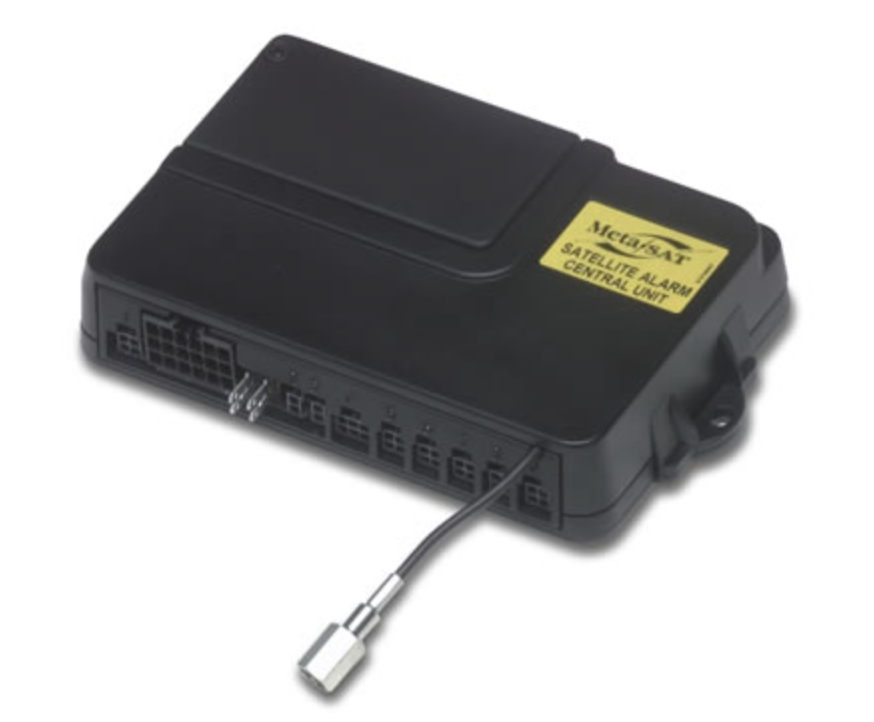
\includegraphics[width=8cm]{esempioScatolaNera.png}
\caption{Esempio di scatola nera\protect\footnotemark}
\label{fig:scatolaNera}
\end{figure}
\footnotetext{Presa da: \url{https://www.drivingtesttips.biz/wp-content/uploads/2016/01/car-insurance-black-box.jpg}}

\subsection{Utilità}
\begin{itemize}
    \item \textbf{Tracciamento GPS}: registra i movimenti del veicolo, inclusi i percorsi effettuati, le velocità raggiunte e le soste. Questo aiuta a localizzare il veicolo in caso di furto e a fornire assistenza immediata in caso di emergenza \cite{khin2018real}.
    \item \textbf{Monitoraggio del comportamento di guida}: registra il comportamento del conducente, come accelerazioni brusche, frenate improvvise, velocità eccessive e svolte pericolose. Questi dati aiutano a valutare lo stile di guida e possono essere utilizzati per migliorare la sicurezza. \cite{hermawan2020acquisition}
    \item \textbf{Supporto in caso di incidenti}: fornisce dati cruciali sugli incidenti, come la velocità al momento dell'impatto e la posizione esatta dell'incidente. Queste informazioni possono essere molto importanti per le indagini post-incidente e per la richiesta di soccorsi. \cite{thompson2010using}
\end{itemize}
\subsection{Importanza}
L'importanza di una black box è data dai benefici che si possono trarre da essa: 
\begin{itemize}
    \item \textbf{Assistenza rapida}: in caso di incidente, la scatola nera può inviare automaticamente la posizione ai servizi di emergenza, riducendo i tempi di risposta.
    \item \textbf{Recupero dei veicoli rubati}: la localizzazione GPS permette di tracciare e recuperare rapidamente veicoli rubati.
    \item \textbf{Polizze assicurative personalizzate}: le compagnie assicurative possono utilizzare i dati registrati per profilare meglio i clienti e offrire polizze personalizzate basate sul comportamento di guida e sull'uso del veicolo.
    \item \textbf{Miglioramento della sicurezza}: i dati raccolti possono essere utilizzati per educare i conducenti su comportamenti di guida sicuri, contribuendo a ridurre il rischio di incidenti. Un’indagine dell’ANIA (Associazione Nazionale delle Imprese Assicurative) ha stabilito che chi installa la black box ha una condotta di guida più responsabile \cite{diminuzioneIncidenti}, un comportamento che quindi fa diminuire la probabilità di provocare sinistri. Lo studio ha rilevato una riduzione della sinistrosità per i veicoli controllati dal congegno quasi doppia rispetto a quella delle auto che non montano il sistema di sorveglianza. 
\end{itemize}
\section{Obiettivi del progetto}
Il principale obiettivo di questo progetto è sviluppare una black box avanzata per veicoli appartenenti ad una flotta di autonoleggio a lungo termine, che si distingua dalle soluzioni tradizionali per la sua capacità di diagnosticare sia il veicolo sia il comportamento del conducente. Le tradizionali black box non solo registrano i dati di viaggio e monitorano le condizioni del veicolo, ma svolgono anche funzioni fondamentali come il monitoraggio costante del veicolo, il tracciamento degli incidenti e la richiesta automatica di assistenza in caso di emergenza. La nostra black box, oltre a queste funzionalità di base, introduce due caratteristiche innovative che ne ampliano ulteriormente le potenzialità.

\vspace{1cm}

La \textbf{prima caratteristica distintiva} della nostra black box è la capacità di rilevare e segnalare tempestivamente sia allarmi critici che non, relativi a problemi meccanici del veicolo e comportamenti inappropriati del conducente. Questo sistema avanzato di diagnostica è in grado di identificare malfunzionamenti interni dell’autovettura, come anomalie nel motore, nonché situazioni di pericolo come la presenza di gas nell'abitacolo. Inoltre, è capace di monitorare e segnalare comportamenti non leciti del conducente, la presenza di fumo nell'abitacolo potrebbe essere un parametro che deve essere rispettato dalla compagnia, guida sotto l'influenza di alcool, utilizzo del veicolo su strade non asfaltate, guida fuori dal territorio nazionale o trasporto di un rimorchio senza autorizzazione.

\vspace{1cm}

La \textbf{seconda caratteristica innovativa} è la generazione automatica di un punteggio di guida per il conducente. Questo voto è calcolato sulla base dei dati raccolti durante la guida, valutando il comportamento al volante del conducente. Il punteggio serve non solo come feedback per il conducente, aiutandolo a migliorare le proprie abitudini di guida, ma potrebbe essere utilizzato dalle compagnie assicurative per offrire polizze più personalizzate e vantaggiose, stimolando il conducente a mantenere uno stile di guida più prudente. È importante sottolineare che questa profilazione del conducente non richiede l'intervento di un esperto lato server remoto, poiché è la stessa black box a elaborare e generare automaticamente il punteggio di guida.

\vspace{1cm}

Il progetto mira a creare una black box che non solo registra e monitora i dati di viaggio e le condizioni del veicolo, ma offre anche un sistema di diagnostica integrato in grado di riconoscere comportamenti inappropriati del conducente ed in grado di valutarlo in base al suo stile di guida; migliorando la sicurezza e l’efficienza del veicolo e contribuendo ad una guida più responsabile e consapevole.

\chapter{Stato dell'arte}
La \textbf{scatola nera}, chiamata anche black-box o EDR, acronimo per Event Data Recorder o, in italiano, registratore di dati di evento, è un dispositivo che registra e trasmette la propria posizione ai satelliti a cui è collegata e altre informazioni come la velocità, le accelerazioni, le decelerazioni, le frenate e la frequenza di attivazione dei sistemi di sicurezza a una centrale operativa.
Quelle che sono comunemente indicate come "scatole nere" sono localizzatori satellitari GPS installati a bordo dell'auto, nate come strumento, ideato dalle assicurazioni, per ridurre le \textbf{frodi assicurative}.
\section{Gestioni attuali di tracking per veicoli}
Unico beneficio del tracking del veicolo è che, grazie al localizzatore GPS, risulta utile in caso di furto: il sistema satellitare facilita il rintracciamento del veicolo qualora venga rubato. Naturalmente il localizzatore GPS gioca un ruolo importante anche nella gestione di un incidente, infatti ne verrà parlato nel prossimo paragrafo.
\section{Gestioni attuali delle emergenze e dei sistemi di allarmi in uso}
\subsection{Vantaggi e Svantaggi nella gestione delle emergenze}
\subsubsection{Vantaggi}
Grazie all'installazione di una black-box sul proprio veicolo e al monitoraggio continuo e tracking di esso, è possibile, in caso di incidente, visualizzare il luogo dell'accaduto immediatamente e ricostruire con precisione la dinamica degli incidenti stradali. Tramite questo strumento le compagnie assicurative sono in grado di ricostruire più facilmente la dinamica di un sinistro stradale. Questo non solo avvantaggia la compagnia, ma anche il guidatore, che vedrà diminuire il tempo per ottenere il risarcimento del danno dato che grazie alla black-box è possibile evitare le lunghe procedure per l'accertamento delle responsabilità in un incidente.
\subsubsection{Svantaggi}
Le black-box attuali sono in grado di registrare anche la velocità del veicolo: in un ipotetico incidente, senza alcun tipo di colpa, se fosse stata registrata una velocità anche poco sopra al limite, si potrebbe riconoscere al guidatore una piccola parte di responsabilità nel sinistro.

\vspace{1cm}

Nei vari contratti di noleggio \cite{hertz_pdf} vengono proposti dei termini e delle condizioni sull'utilizzo dell'autovettura, quali ad esempio non utilizzare il veicolo: 
\begin{itemize}
    \item  sotto l'influsso di alcool.
    \item da persone sprovviste di patente o con validità scaduta.
    \item fuori strada o su strade inadatte.
    \item per recarsi all'estero salva preventiva autorizzazione concessa dal noleggiante.
    \item per trainare o spingere qualsiasi altro veicolo, rimorchio o altro oggetto senza consenso del noleggiatore.
\end{itemize}
Tutti questi obblighi vengono citati all'interno del contratto assicurativo, non è possibile però stabilire se uno tra questi divieti non dovesse essere rispettato.

\section{Soluzioni esistenti per la profilazione guidatori}
Alcune grandi compagnie di assicurazioni, quali ad esempio \textbf{Generali}, propongono il \textbf{servizio stile di guida} che permette di ottenere ulteriori sconti sulla polizza negli anni a seguire \cite{Generali}. Tengo a precisare la parola "ulteriori" dato che già l'installazione di una black-box prevede uno sconto, compreso tra il 15/20\%, sul totale dell'assicurazione.

\section{Trattamento dei dati personali registrati}
Il Regolamento europeo vieta espressamente che la scatola nera registri conversazioni o usi i dati sensibili del guidatore, consentendo così l’anonimato del conducente e l’accesso ai dati solo in caso di collisione \cite{RegolamentoEU}.

\section{Quanto è comune la scatola nera in Italia?}
L'uso della scatola nera in Italia inizia ad essere rilevante. Il trend di crescita non si è mai interrotto negli ultimi 10 anni e la percentuale di auto dotate di black-box sono passate dal 6\% del 2013 al 23,2\% del 2020 (primo semestre)  \cite{Telepass}. Uno dei principali motivi di tale gradimento sono gli sconti sulle teriffe delle varie assicurazioni. I dati del 2021 del report IVASS confermano una diffusione più alta nei centri urbani del Sud Italia, come Caserta (65,5\%), Napoli (52,5\%) e Reggio Calabria (38,6\%). Le percentuali calano sotto il 10\% nelle città e nelle province del Nord come Udine (9\%), Trento (8\%), Belluno (7,3\%) e Bolzano (4,4\%).

\chapter{Funzionalità del sistema}
\section{Monitoraggio}
Il monitoraggio consiste nella raccolta dati di alcuni parametri provenienti dal lettore OBD e da alcuni sensori installati sulla black box. 
Il motivo per cui si è scelto di monitorare lo stato del veicolo è quello di ottenere una visione completa della sua salute. In particolare, i dati che vengono registrati sono l'accelerazione misurata grazie ad un accelerometro, utile per analizzare il comportamento dinamico del veicolo. Il sensore di alcool mi permette di rilevare la presenza di vapori alcolici nell'abitacolo, garantendo un ambiente sicuro; per assicurare una qualità dell'aria adeguata all'interno del veicolo, utilizzo un sensore specifico che rileva vari inquinanti, il modulo GPS fornisce coordinate precise, fondamentali sia per la tracciabilità del veicolo in caso di furto, sia per analizzare i percorsi abituali. Viene inoltre monitorata  costantemente la temperatura del liquido di raffreddamento e dell'olio motore grazie allo scanner OBD. Inoltre, vengono registrati la coppia del motore per valutare le sue prestazioni e il voltaggio della batteria per prevenire problemi elettrici.
Infine, il sensore del livello del carburante mi permette di tenere traccia dell'autonomia del veicolo. 
\section{Tracking}
Questa funzionalità del sistema viene adoperata per localizzare i veicoli della flotta \cite{al2012hybrid}. Il sistema di tracking è in grado di generare la posizione esatta del veicolo usando due parametri, latitudine e longitudine; i dati di geolocalizzazione, per ogni slot temporale di 5 minuti, vengono trasferiti al server remoto della centrale operative dell'autonoleggio; a posteriori potrebbero essere utilizzati per visualizzare i percorsi abituali del cliente o il percorso effettuato un preciso giorno. Il sistema di tracking è utile soprattutto in caso di furto del veicolo.
L'antenna GPS e il ricevitore GPS ricevono informazioni dal satellite nel formato NMEA (National Marine Electronics Association), queste vengono processate dall'esp32 e trasmesse al server remoto via GSM, il server una volta ricevuto i dati li memorizza in locale per analisi future. 

\begin{figure}[h] \centering
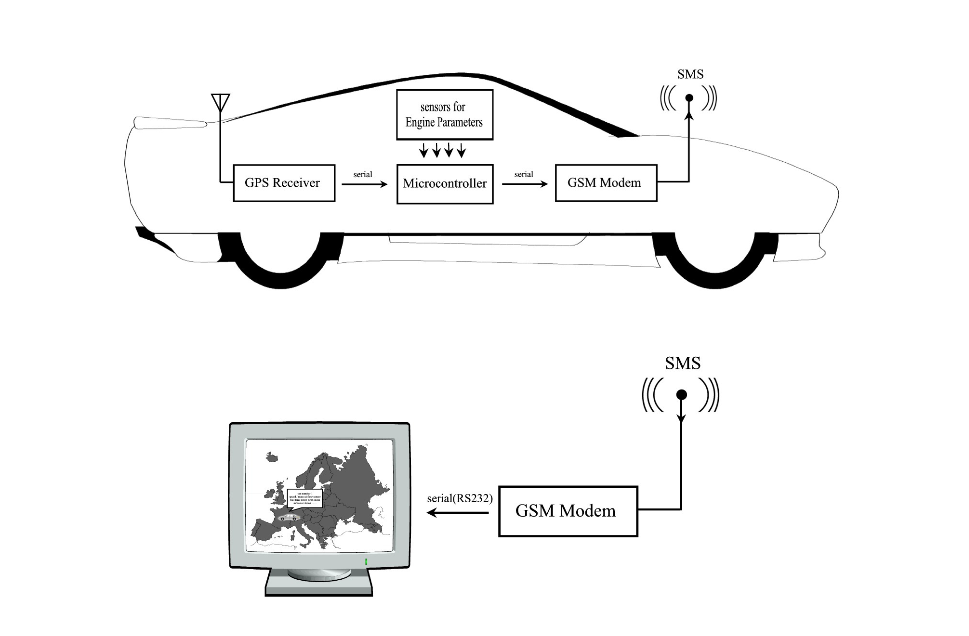
\includegraphics[width=8cm]{tracking.png}
\caption{L'architettura del sistema: localizzazione GPS e modulo GSM\protect\footnotemark}
\label{fig:trackingGPS}
\end{figure}
\footnotetext{Presa da: \url{https://www.researchgate.net/profile/Mohammad-Alkhedher/publication/51989090/figure/fig5/AS:668830275760151@1536472972974/The-system-architecture-GPS-tracking-and-GSM-modules.ppm}}

In molti casi il GPS potrebbe darci una risposta errata o non sufficientemente precisa, dovuta a molti fattori esterni, quali condizioni del tempo atmosferico e dell'ambiente che circonda il veicolo.

\section{Segnalazione di allarmi}
Il meccanismo di segnalazione allarmi prevede 3 diversi tipi di dinamiche che verranno presentate in dettaglio nei seguenti paragrafi. 
\subsection{Incidente}
L'assistenza incidente tratta la dinamica relativa ad un incidente stradale, inviando le coordinate GPS ed un insieme di informazioni utili ad una stazione remota dell'autonoleggio, sarà compito della stazione avvisare i soccorsi che andranno poi a recarsi nel preciso punto di impatto. 
\begin{figure}[h] \centering
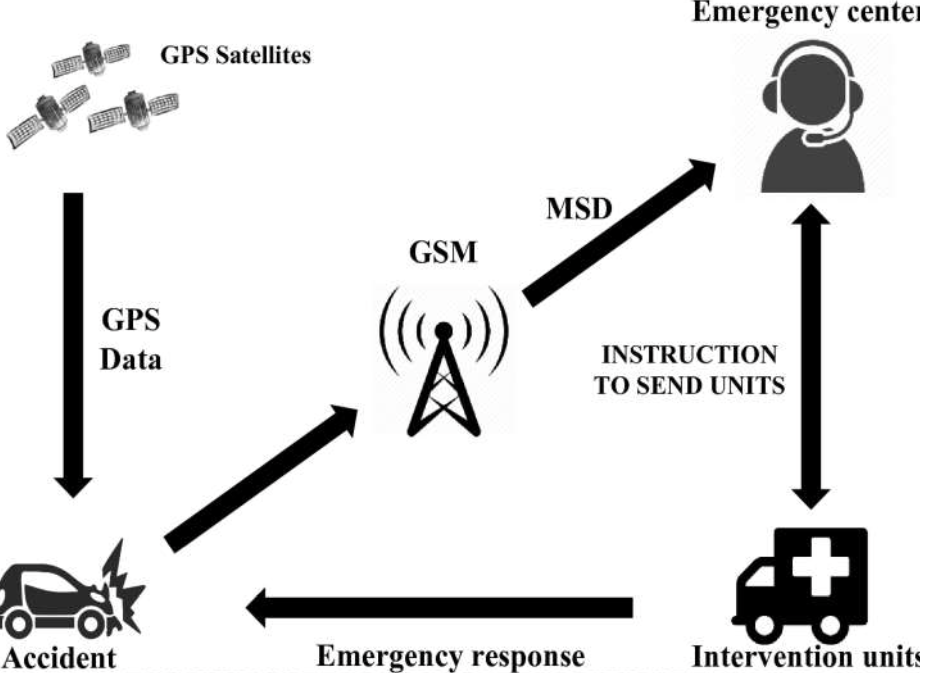
\includegraphics[width=8cm]{incidente.png}
\caption{Schema situazione di emergenza dovuta ad un incidente\protect\footnotemark}
\label{fig:emergenzaIncidente}
\end{figure}
\footnotetext{Presa da: \url{https://www.researchgate.net/publication/51989090_Hybrid_GPS-GSM_localization_of_automobile_tracking_system}}

Sostanzialmente il meccanismo si divide in due fasi: \textbf{rilevamento} e \textbf{notifica} vedi figura \ref{fig:rilevamentoInvioIncidente}.

\begin{figure}[h]
    \centering
    \begin{tikzpicture}[node distance=2cm]

    % Nodi del diagramma
    \node (start) [startstop] {Start};
    \node (readsensor) [process, below of=start] {Read the status of sensor};
    \node (readgps) [process, below of=readsensor] {Read the data from GPS};
    \node (decision) [decision, below of=readgps, yshift=-1cm] {Sensor is triggered?};
    \node (sendSMS) [process, right of=decision, xshift=4cm] {Send SMS using GSM};
    \node (end) [startstop, below of=sendSMS] {End};

    % Frecce del diagramma
    \draw [arrow] (start) -- (readsensor);
    \draw [arrow] (readsensor) -- (readgps);
    \draw [arrow] (readgps) -- (decision);

    % Etichette "Yes" e "No"
    \node at ($(decision.west)!-0.2!(readsensor.east)$) [yshift=3cm] {No};
    \node at ($(decision.east)!0.5!(sendSMS.west)$) [yshift=0.3cm] {Yes};

    \draw [arrow] (decision) -| ++(-3,0) |- (readsensor);
    \draw [arrow] (decision) -- (sendSMS);
    \draw [arrow] (sendSMS) -- (end);

    \end{tikzpicture}
    \caption{Diagramma di flusso per il monitoraggio dell'accelerometro ed eventuale invio SMS}
    \label{fig:rilevamentoInvioIncidente}
\end{figure}

I sensori maggiormente coinvolti sono l'accelerometro, il GPS e il dato relativo alla velocità del veicolo proveniente dalla rete can bus. Nella fase di campionamento, l'accelerometro contina ad estrarre informazioni relative alla forza G speriementata dagli occupanti. Il GPS, nella fase di notifica, è utile per inviare le coordinate alla stazione remota. Infine la velocità del veicolo, coinvolta sempre in fase di notifica, viene mandata alla stazione remota e può essere utilizzata per future ricostruzioni/analisi dell'incidente. \cite{shubham2021survey}

Per il rilevamento di una situazione di incidente posso utilizzare un accelerometro, in un evento del genere la black box subirà la stessa accelerazione degli occupanti del veicolo. La forza G che si ricava dall'accelerazione deve essere ragionevolmente alta per un incidente, per questo non vengono considerati incidenti se tutte le accelerazioni sono inferiori a 4G \cite{thompson2010using}. Infatti sulle auto gli airbag non vengono altro che azionati dal superamento di una certa soglia di accelerazione. Come secondo filtro viene utilizzato un sistema di conferma per evitare i falsi positivi, all'utente vengono concessi 30 secondi per annullare il rilevamento della situazione di incidente, terminato questo breve periodo, il messaggio verrà trasmetto al server remoto in automatico, in caso di annullamemto si ritornerà ad una situazione di partenza

\begin{figure}[h]
    \centering
    \begin{tikzpicture}[node distance=2cm, every node/.style={font=\small}]

    % Nodi del diagramma
    \node (start) [startstop] {Start};
    \node (readdata) [process, below of=start] {Read data};
    \node (gforcetriggered) [decision, below of=readdata] {G force triggered?};
    \node (incidentdetection) [process, below of=gforcetriggered, yshift=-0.5cm] {Rilevamento incidente};
    \node (userabort) [decision, below of=incidentdetection, yshift=-0.5cm] {User abort?};
    \node (sendSMS) [process, right of=userabort, xshift=3cm] {Send accident SMS};
    \node (end) [startstop, below of=sendSMS] {End};

    % Etichette "Yes" e "No"
    \node at ($(gforcetriggered.east)!0.5!(readdata.east)$) [xshift=1.3cm] {No};
    \node at ($(gforcetriggered.south)!0.5!(incidentdetection.north)$) [xshift=0.5cm] {Yes};
    \node at ($(userabort.east)!0.5!(sendSMS.west)$) [yshift=0.3cm] {No};
    \node at ($(readdata.south)!0.5!(userabort.north)$) [xshift=-3.2cm] {Yes};

    % Frecce del diagramma
    \draw [arrow] (start) -- (readdata);
    \draw [arrow] (readdata) -- (gforcetriggered);
    \draw [arrow] (gforcetriggered) -- (incidentdetection);
    \draw [arrow] (incidentdetection) -- (userabort);
    \draw [arrow] (userabort.west) -| ++(-1,0) |- (readdata.west);
    \draw [arrow] (gforcetriggered.east) -| ++(0.5,0) |- (readdata.east);
    \draw [arrow] (userabort) -- (sendSMS);
    \draw [arrow] (sendSMS) -- (end);

    \end{tikzpicture}
    \caption{Diagramma di flusso per il rilevamento di incidenti e invio SMS}
    \label{fig:diagramma-flusso-incidenti}
\end{figure}

\begin{flushleft}
    \begin{minipage}[t]{0.3\textwidth}
        \scriptsize
        \begin{align*}
            \text{Incidente} &= I \\
            \text{Accident\_threshold} &= 1 \\
        \end{align*}
    \end{minipage}
    \vspace{0.5cm} % Aggiunge uno spazio verticale tra la legenda e la formula
    \begin{minipage}[t]{0.7\textwidth}
        \begin{align*}
            I &= 
            \begin{cases}
                1 & \text{se } \left( \frac{\text{Accelerazione}}{4G} \right) \geq \text{Accident\_threshold} \text{ \&\& } \neg\text{userAbort} \\
                0 & \text{altrimenti}
            \end{cases}
        \end{align*}
    \end{minipage}
\end{flushleft}

A seguito dell'incidente le informazioni che possono essere trasmesse sono la \textbf{forza G} per capire quanto effettivamente è stato forte l'impatto, la \textbf{velocità del veicolo} per capire a quanto stava andando, le \textbf{coordinate GPS} per individuare il luogo in cui è avvenuto l'incidente e in che \textbf{momento} è avvenuto.

\subsection{Assistenza}
Il sistema include un pulsante che permette al conducente di comunicare direttamente con il server remoto (la centrale dell'autonoleggio), inviando un messaggio tramite GSM in caso di necessità.
\subsection{Rilevamento allarmi}
Il rilevamento di allarmi consiste nell'avvertire il conducente e la centrale dell'autonoleggio di alcuni sistemi del veicolo non funzionanti e di alcuni comportamenti non corretti da parte del conducente. Per gestire tale situazione, la black box viene dotata di 3 led per indicare diversi tipi di situazioni e per suggerire al cliente il corretto comportamento da intraprendere nel caso dell'accensione di una spia (led) indicante una situazione di avvertimento. 
\begin{itemize}
    \item Il led \textbf{verde} indica che il veicolo \textbf{funziona correttamente} e il \textbf{comportamento} del conducente è \textbf{corretto}.
    \item Il led \textbf{giallo} indica un \textbf{avvertimento}, se vengono rilevati problemi di poca rilevanza o eseguite azioni non lecite viene azionato il led, dopo aver superato una certa soglia di tolleranza indicante il numero di volte in cui è stato rilevato il problema o eseguita l'azione non lecita, viene avvertita la centrale operativa. Il motto di questa spia è: se un problema di poca rilevanza o un'azione non lecita persistono, avverto la centrale.
    \item Il led \textbf{rosso} indica una situazione di \textbf{pericolo}, in questo caso la centrale operativa viene avvertita immediatamente.
\end{itemize}

Di seguito verranno proposte le dinamiche delle situazioni per le quali viene attivata una spia gialla piuttosto che una rossa.

\subsubsection{Non critici (led giallo)}

\begin{itemize}
    \item Divieto di fumo all'interno dell'abitacolo per il mantenimento di un ambiente pulito e privo di odori sgradevoli per i successivi clienti.
    \item Rilevamento guida su terreni non adatti: fuoristrada o percorsi non asfaltati sono vietati al conducente per evitare danni al veicolo. 
    \item Rilevamento guida su aree geografiche non percorribili: non è possibile recarsi ovunque con il veicolo della compagnia, ad esempio fuori da una certa nazione, o da un loro insieme.
    \item Rilevamento attività di trasporto/rimorchio: non è possibile trainare qualsiasi tipo di rimorchio con il veicolo a noleggio.
\end{itemize}

\subsubsection{Critici (led rosso)}

\begin{itemize}
    \item Temperatura anomala olio motore: il motore non lavora nel suo range di    temperatura e potrebbe guastarsi.
    \item Temperatura liquido refrigerante: una temperatura troppo alta potrebbe danneggiare componenti del motore, causando gravi guasti.
    \item Coppia motore anomala: mantenere la coppia motore entro limiti ottimali è essenziale per garantire prestazioni efficienti e sicure del veicolo. prevenendo l'usura prematura del motore e della trasmissione. Se la coppia è troppo bassa, si rischia una scarsa accelerazione; se troppo alta, si può verificare un eccessivo consumo di carburante e possibili danni meccanici.
    \item Monitoraggio della qualità dell'aria nell'abitacolo: utile per prevenire qualunque perdita di gas proveniente dai vari impianti dell'automobile, prevenendo così incendi.
    \item Rilevamento presenza di alcool: non è consentito al conducente mettersi alla guida in stato di ebrezza. Questa attività può essere monitorata attraverso un sensore che rileva la presenza di etanolo nell'ambiente. \cite{ahmar2021road}
    \item Distanza di frenata anomala: analizzando dati di accelerazione, velocità e spazio percorso è possibile rilevare situazioni in cui la distanza di frenata è significativamente più lunga, ciò può indare un problema al sistema frenante o all'aderenza dei pneumatici.
    \item Consumo anomalo di carburante: monitorando il consumo di carburante del veicolo e confrontandolo con i modelli di consumo attesi è possibile rilevare anomalie che potrebbero indicare problemi al motore.
\end{itemize}

\section{Profilazione del comportamento del guidatore}
\label{sec:AnalisiProfilazione}
Nel quadro del progetto dell'analisi della profilazione guida, sfruttiamo tecnologie di acquisizione dati per ottenere una comprensione dettagliata del comportamento del guidatore. A tale scopo, viene fatto uso di due principali fonti di informazioni: i \textbf{dati provenienti dal sistemna diagnostico di bordo OBD-II} e quelli registarti da un \textbf{accelerometro}. Questi dispositivi forniscono una vasta gamma di dati in tempo reale, quali ad esempio velocità, accelerazione, decelerazione (frenata) e angoli di sterzata, consentendo di valutare numerosi aspetti relativi alla guida. Attraverso l'analisi approfondita di tali dati, siamo in grado di creare profili individuali dei guidatori e identificare modelli di comportamento distintivi che influenzano la sicurezza, l'efficienza e l'affidabilità del veicolo. Nel corso di questo paragrafo esploreremo come l'integrazione di queste tecnologie ci permetta di ottenere informazioni preziose per migliorare l'esperienza di guida e ottimizzare le operazioni di gestione della flotta.

\vspace{1cm} 

I principali parametri che vengono catturati per l'analisi del guidatore sono: \textbf{rpm} ovvero i giri motore al minuto, la \textbf{velocità dell'auto}, il \textbf{carico del motore} e la \textbf{posizione della valvola farfalla}, provenienti dalla rete CAN-BUS presente all'interno del veicolo, \textbf{accelerazione}, \textbf{decelerazione} e \textbf{sterzate} provengono invece dall'accelerometro. Una volta che la black box riceve i valori dei parametri, essa è in grado di analizzarli e riconoscere situazioni riconducibili ad una guida impropria. Ogni 24h tali dati vengono adoperati per calcolare un punteggio di guida compreso tra 0 e 1. Questo punteggio potrebbe essere utilizzato dalla compagnia per varie finalità, come ad esempio fornire incentivi ai guidatori che adottano comportamenti di guida più sicuri. Ecco le principali fasi del sistema proposto \ref{diagrammaFlussoProfilazione}:

\vspace{1.2cm}

\begin{figure}[h!]
\centering
\begin{tikzpicture}

% Definizione dei nodi con posizionamento manuale
\node (data_sensing) [process] {Data sensing};
\node (data_acquisition) [process, right=1cm of data_sensing] {Data acquisition};
\node (data_processing) [process, right=1cm of data_acquisition] {Data processing};
\node (data_storage) [process, right=1cm of data_processing] {Storage vote};

% Connessione tra i nodi
\draw [arrow] (data_sensing) -- (data_acquisition);
\draw [arrow] (data_acquisition) -- (data_processing);
\draw [arrow] (data_processing) -- (data_storage);

\end{tikzpicture}
\caption{Diagramma di flusso dei dati}
\label{diagrammaFlussoProfilazione}
\end{figure}

\vspace{0.8cm}

ECU è l'unità centrale di controllo del veicolo dove sono collegati tutti i vari attuatori e sensori del veicolo: motore, aria condizionata, livello carburante... Lo scanner OBD-II trasmette i dati dalla ECU alla board via Bluetooth. La board processa i dati ed è in grado di generare uno score del guidatore. Il punteggio [0,1] viene calcolato considerando:

\begin{itemize}
    \item Le accelerazioni e decelerazioni brusche. \cite{fazeen2012safe}
    \item Le strerzate sia a sinistra che a destra brusche. \cite{fazeen2012safe}
    \item Il rapporto (relativo) di velocità del veicolo con i giri del motore che deve essere compreso tra i valori di [0.9,1.3] per una buona guida. \cite{chen2015driving}
    \item Il rapporto (relativo) tra la valvola a farfalla e i giri del motore che deve essere compreso tra i valori di [0.9,1.3] per una buona guida. \cite{chen2015driving}
    \item Il carico del motore che deve essere compreso tra il 20\% e il 50\% per una buona guida. \cite{chen2015driving}
    \item Gli eccessi di velocità data dalla differenza tra i limiti imposti dalla legge e quelli reali del veicolo.
\end{itemize}

\begin{lstlisting}
// Implementazione task relativo alla profilazione guida
void profilazioneCallback() {
  campionamento_Profilazione++;
  sensors_event_t a, g, temp;
  mpu.getEvent(&a, &g, &temp);

  float x = a.acceleration.x;
  float y = a.acceleration.y;

  // Accelerazioni / decelerazioni brusche
  if ((x / FORZA_G) > (ACCELERAZIONE_BRUSCA) || (x / FORZA_G) < (DECELERAZIONE_BRUSCA)) {
    nRilevamentiAccDecBrusche++;
  }
  // Sterzate sinistra e destra brusche
  if ((y / FORZA_G) > (STERZATA_DX_BRUSCA) || (y / FORZA_G) < (STERZATA_SX_BRUSCA)) {
    nRilevamentiSterzateBrusche++;
  }
  // Rapporto v su giri motore
  float fatt1 = ((kph / MAX_SPEED_CAR) / (rpm / MAX_RPM_CAR));
  if ((fatt1 < RANGE_INF) || (fatt1 > RANGE_SUP)) {
    nRilevamentiFatt1++;
  }
  // Rapporto posizione della valvola a farfalla su giri motore
  float fatt2 = ((throttle / 100) / (rpm / MAX_RPM_CAR));
  if ((fatt2 < RANGE_INF) || (fatt2 > RANGE_SUP)) {
    nRilevamentiFatt2++;
  }
  // Carico motore
  if ((load < LOAD_MIN) || (load > LOAD_MAX)) {
    nRilevamentiCaricoMotoreOutOfRange++;
  }
  if (campionamento_Profilazione == MAX_CAMPIONAMENTI_PROFILAZIONE) {  
    updateCampionamentoProfilazione();
  }
}
\end{lstlisting}
\vspace{0.5cm}
Per quanto riguarda il primo e il secondo punto è possibile utilizzare un accelerometro a 3 assi utile per rilevare  le accelerazioni/decelerazioni e le sterzate improvvise: 

\begin{table}[h!]
  \centering
  \begin{tabular}{|c|c|c|}
    \hline
    \textbf{Asse} & \textbf{Direzione} & \textbf{Azione/Evento} \\
    \hline
    x & anteriore/posteriore & accelerazione/decelerazione (frenata) \\
    \hline
    y & sinistra/destra & sterzata \\
    \hline
    z & su/giù & strada dissestata \\
    \hline
  \end{tabular}
  \caption{Descrizione degli assi dell'accelerometro utilizzati nell'ambito della profilazione del guidatore}
  \label{tab:tabellaAccelerometro}
\end{table}

\begin{figure}[h]
  \centering
  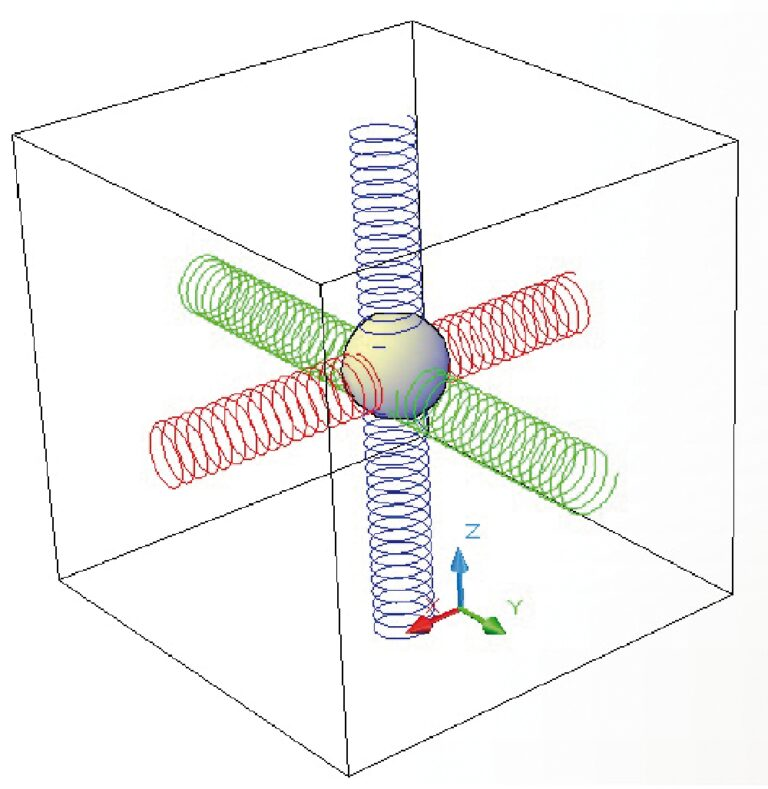
\includegraphics[width=8cm]{Accelerometro.jpg}
  \caption{Modello meccanico di un accelerometro a 3 assi}
  \label{fig:accelerometro}
\end{figure}
\footnotetext{Presa da: \url{https://futuranet.it/wp-content/uploads/2023/01/Figura-4-6-768x789.jpg}}

Il terzo e quarto punto sono invece calcolabili per via analitica raccogliendo dati provenienti dall'OBD-II; per quanto riguarda l'ultimo punto (carico del motore espresso in \%) non si ha bisogno di alcuna manipolazione dei dati in quanto essi provengono direttamente dalla rete CAN-BUS.

Per valutare il comportamento del guidatore di seguito vengono mostrati i vari livelli di punteggio del guidatore:

\begin{table}[h!]
  \centering
  \begin{tabular}{|c|c|}
    \hline
    \textbf{Driver score} & \textbf{Driving behaviour} \\
    \hline
    \(< 0.10\) & safe \\
    \hline
    0.1 - 0.18 & modest \\
    \hline
    0.19 - 0.38 & moderate risk \\
    \hline
    0.39 - 0.56 & risk \\
    \hline
     0.57 - 0.75 & reckless \\
    \hline
     \(> 0.75\) & critical \\
    \hline
  \end{tabular}
  \caption{Tabella di valutazione del conducente}
  \label{tab:tabellaValutativa}
\end{table}

Il punteggio del guidatore è inteso come la probabilità di rischio di procurare un incidente a seguito del viaggio osservato, pertanto sarà compreso tra 0 e 1.

\chapter{Implementazione del sistema}
\section{Architettura}

\subsection{Componenti hardware utilizzati}

Il microcontrollore principale utilizzato per l'elaborazione dei dati e la comunicazione con le periferiche è un \textbf{ESP-WROOM-32}, un chip di basso costo e bassa potenza con integrati i moduli WiFi e Bluetooth. 
Viene utilizzato un \textbf{Display LCD 16x2} utile per interagire con l'utente e avvisarlo in caso sia presente qualche problema al veicolo o viene rilevato qualche comportamento anomalo. \textbf{MQ-2} e \textbf{MQ-3} vengono adoperati come sensori per il rilevamento di gas e alcool, un \textbf{bottone} viene adoperato per la richiesta di assistenza alla centrale operativa, dei \textbf{led}, presenti in 3 colorazioni: rosso, giallo e verde, vengono adoperati come spie per richiamare, con un effetto visivo, all'attenzione dei possibili scenari che si potrebbero verificare. 
Un modulo \textbf{GPS GY-NEO-6M NEO6MV2} utile per le funzionalità di tracking e monitoraggio, un \textbf{accelerometro GY-521 MPU6050} utile per la profilazione del guidatore, o per segnalare un incidente e per concludere un modulo \textbf{RTC real-time-clock} utile per mantenere un orario anche quando il sistema non è sotto connessione WiFi e/o è spento.

\begin{figure}[h]
  \centering
  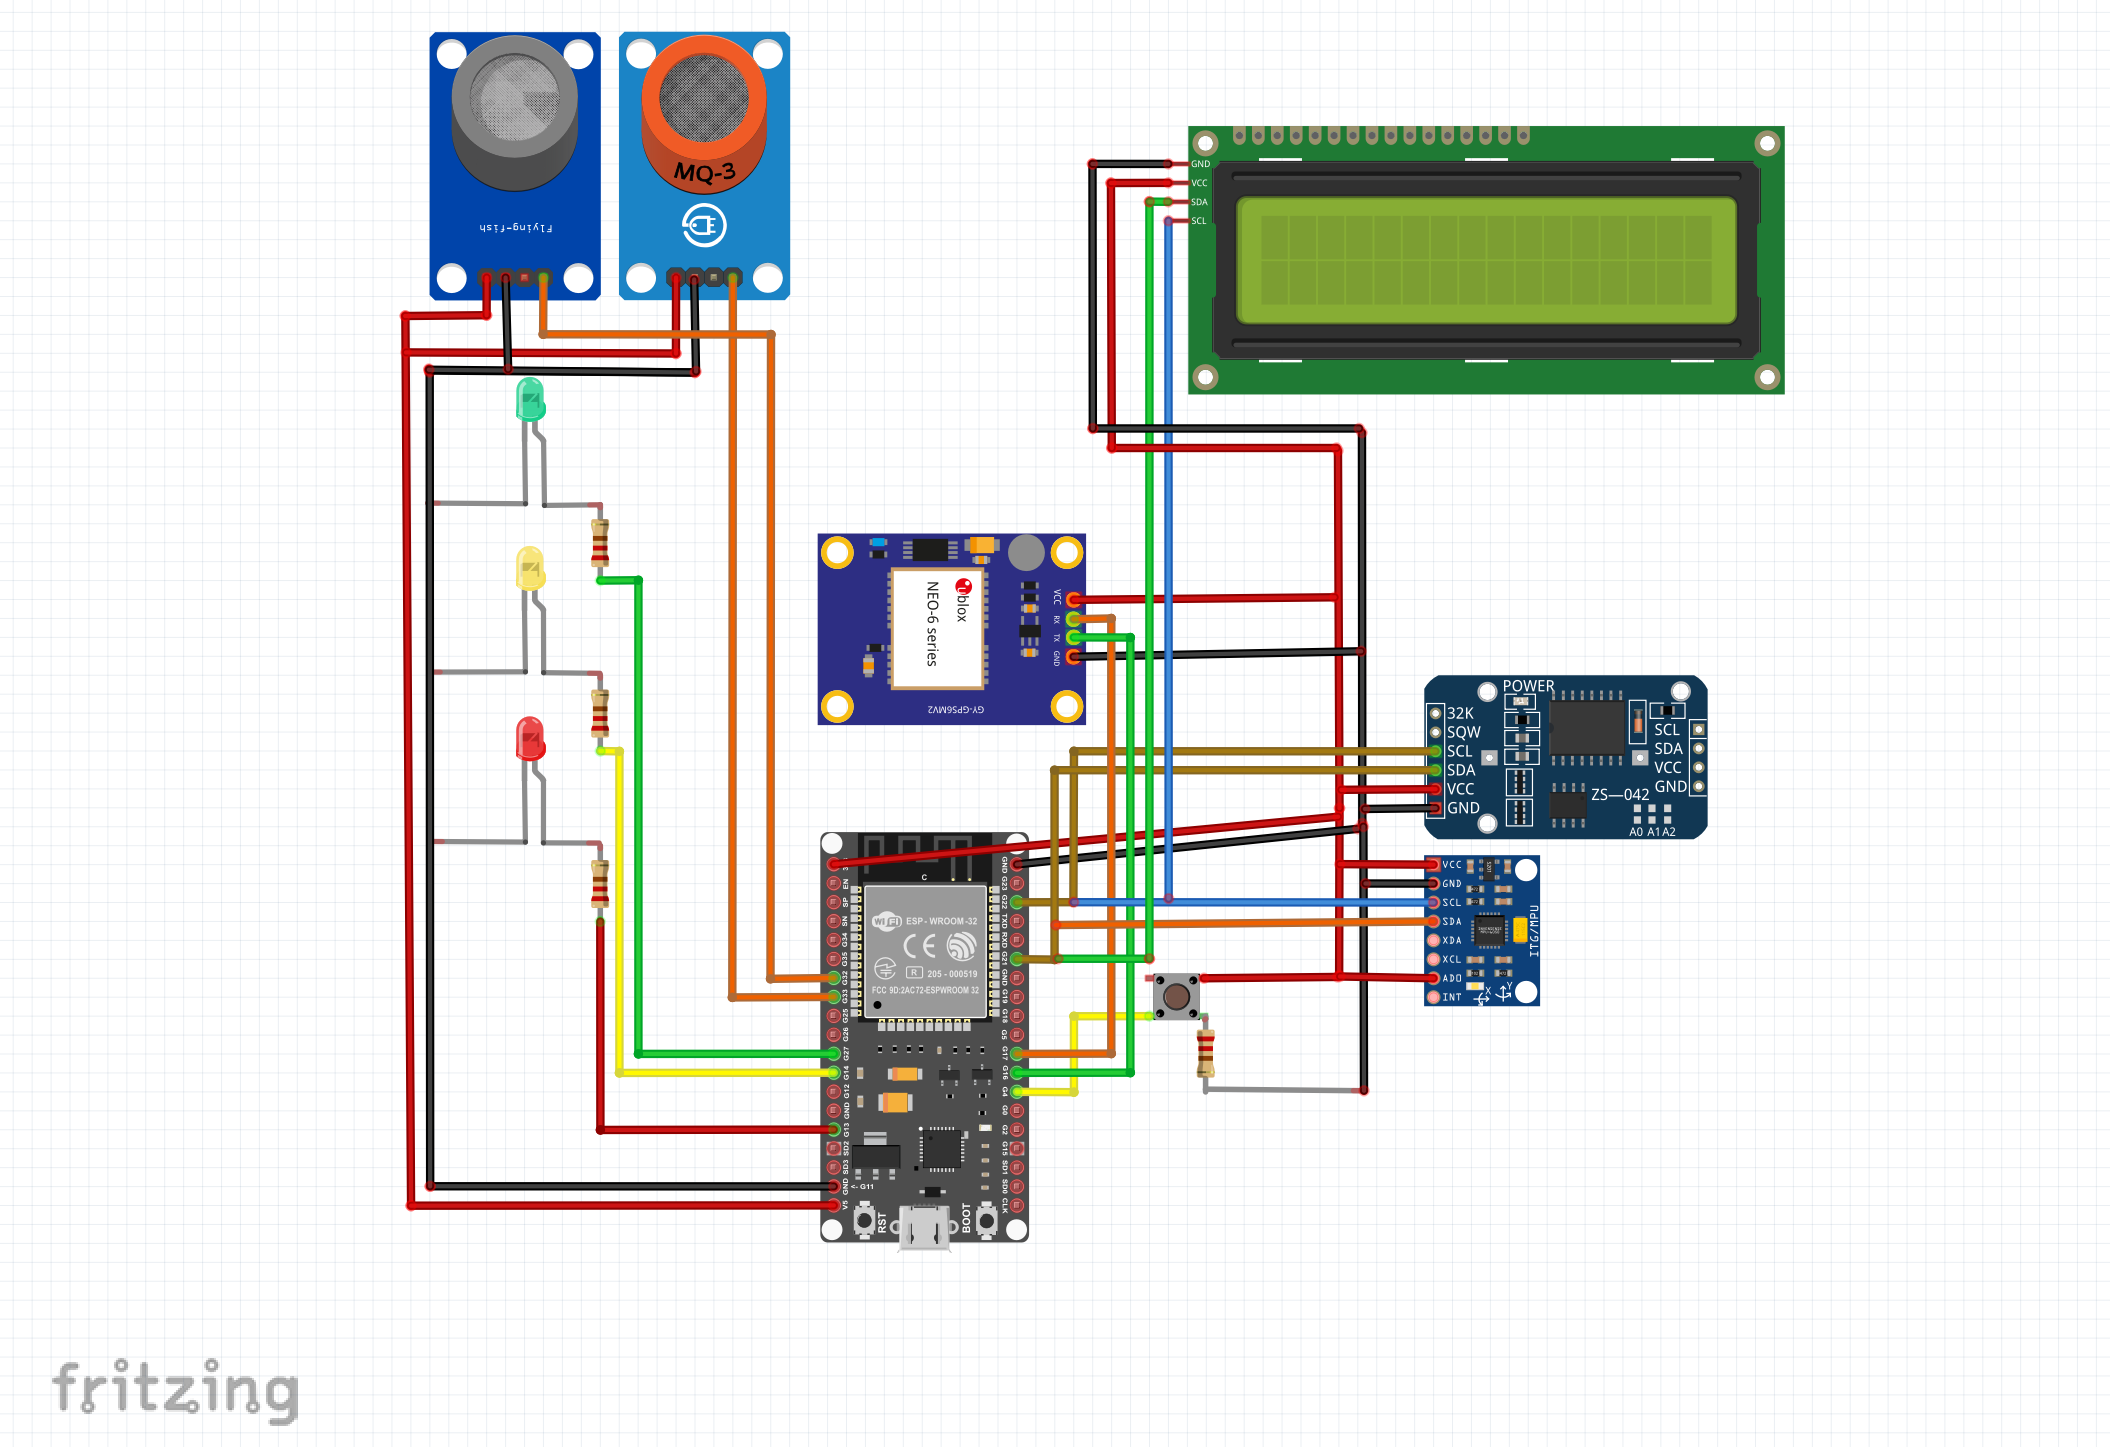
\includegraphics[width=12cm]{circuito_logo.png}
  \caption{Schema di connessione dei vari componenti hardware della black box}
  \label{fig:schemaCircuito}
\end{figure}

\subsection{Software e librerie utilizzate}
Il codice è stato sviluppato sull'Arduino IDE, una piattaforma open-source che rende semplice scrivere codice e caricarlo direttamente nelle varie board scelte all'interno di una sezione apposita. Il linguaggio di programmazione utilizzato all'interno dell'IDE si chiama "Arduino programming language", la sintassi è molto simile ai linguaggi C/C++, ma i costrutti puù complessi come puntatori o la programmazione orientata agli oggetti vengono messi in secondo piano \cite{sistemiEmbeddedAtrent}. Oltre a fornire i costrutti standard di un linguaggio imperativo, dato il contesto applicativo dei sistemi di controllo (sensoristica e attuatoristica), offre funzionalità legate alla gestione dei segnali: I/O digitale e analogico, interrupt su eventi hardware e accesso al clock (inteso proprio come tempo trascorso dall'accensione).

Le librerie utilizzate per lo sviluppo del progetto si possono divedere in tre categorie:

\begin{itemize}
    \item Le librerie dedicate all'interazione con i vari sensori, ad esempio \textbf{TinyGPSPlus.h} per il GPS, \textbf{Adafruit\_MPU6050.h} per l'accelerometro, \textbf{LiquidCrystal\_I2C.h} per il display, e \textbf{time.h, sntp.h, RTClib.h} per l'RTC.
    \item Le librerie dedicate alla gestione interna del filesystem, ad esempio \textbf{LittleFS.h} per la gestione del filesystem e \textbf{sqlite3.h} per la creazione di database e iterazione con essi.
    \item Le librerie dedicate alla comunicazione con i componenti esterni, ad esempio \textbf{"BluetoothSerial.h"} e \textbf{"ELMduino.h"} che consentono la comunicazione bluetooth tra ESP32 e lettore scanner OBD.
\end{itemize}

\section{Scelte progettuali}
\subsection{Filesystem}
Nel filesystem dell'esp32 viene creato un database (dati.db) all'interno del quale sono presenti 5 tabelle, utili per la gestione di tutti gli eventi previsti dalla black-box. Per interagire con il db viene utilizzato SQLite, una libreria scritta in linguaggio C che implementa un motore di database SQL piccolo, veloce, autonomo, ad alta affidabilità e completo. SQLite è il motore di database più utilizzato al mondo. SQLite è integrato in tutti i telefoni cellulari e nella maggior parte dei computer ed è integrato in innumerevoli altre applicazioni utilizzate ogni giorno \cite{sqliteWhentoUse}. SQLite è particolarmente adatto per l'uso in telefoni cellulari, set-top box, televisori, console di gioco, fotocamere, orologi, elettrodomestici da cucina, termostati, automobili, macchine utensili, aeroplani, sensori remoti, droni, dispositivi medici e robot: \textbf{"internet of things"}.
Di seguito le tabelle di memorizzazione dati dell'intero sistema con qualche esempio di dato memorizzato:

\paragraph{Tabella t1}
\begin{table}[h!]
  \centering 
  \begin{adjustbox}{max width=\textwidth}
    \begin{tabular}{|c|c|c|c|c|c|c|}
      \hline
      \textbf{nomeSensore} & \textbf{valore} & \textbf{tipoDato} & \textbf{unitàMisura} & \textbf{timestamp} & \textbf{synchronised} & \textbf{Priority} \\
      \hline
      TEXT & TEXT & TEXT & TEXT & INTEGER (seconds since epoch) & INTEGER (boolean) & INTEGER \\
      \hline
      "Liquido raffreddamento" & "98" & "INTEGER" & "°C" & 1715786497 & 0 & 3 \\
      \hline
      "Voltaggio batteria" & "12.3" & "FLOAT" & "Volt (V)" & 1715269497 & 1 & 8 \\
      \hline
    \end{tabular}
  \end{adjustbox}
  \caption{Tabella "t1" dati relativi al monitoraggio del veicolo}
  \label{tab:t1 monitoraggio}
\end{table}
Il campo \textbf{timestamp} indica il numero di secondi trascorsi dall'epoc (01/01/1970).

\paragraph{Tabella t2}
\begin{table}[h!]
  \centering 
  \begin{adjustbox}{max width=\textwidth}
    \begin{tabular}{|c|c|c|c|c|c|c|}
      \hline
      \textbf{nomeSensore} & \textbf{tempoStorage} & \textbf{variabile} & \textbf{fattIncr} & \textbf{soglia} & \textbf{tMin} & \textbf{tMax} \\
      \hline
      TEXT & INTEGER & INTEGER & INTEGER & INTEGER & INTEGER & INTEGER \\
      \hline
      "Olio motore temp" & "45" & "1" & "15" & 0.25 & 45 & 600 \\
      \hline
      "Coordinate GPS" & "30" & "0" & NULL & NULL & NULL & NULL \\
      \hline
    \end{tabular}
  \end{adjustbox}
  \caption{Tabella "t2" tempo di campionamento}
  \label{tab:t2 campionamento}
\end{table}
Il campo \textbf{tempoStorage} indica ogni quanto memorizzare il valore, \textbf{variabile} indica se il tempo di storage può cambiare, \textbf{fattIncr} ci dice di quanto aumentare o diminuire il tempoStorage, \textbf{soglia} delimita se i dati campionati sono omogenei, ovvero minori di essa, oppure eterogenei, maggiori di essa (fai approfondimento statistico), infine \textbf{tMin} e \textbf{tMax} sono i corrispettivi upper e lower bound per il tempo di storage.

\textbf{Logica del tempo di campionamento:} se dopo una serie di letture (n ad esempio) i dati hanno una bassa deviazione standard, ovvero sono molto simili tra di loro, memorizzo i dati del veicolo con una frequenza minore, aumentando il tempo di storage di un certo fattore, presente nella tabella di campionamento (\textbf{fattIncr}); se la deviazione standard è alta, significa che i dati sono abbastanza differenti tra di loro e li monitoro con una frequenza maggiore. Naturalmente vengono posti dei lower e upper bound per il tempo di memorizzazione entro i quali il tempo stesso può variare.

\paragraph{Tabella t3}
\begin{table}[h!]
  \centering 
  \begin{adjustbox}{max width=\textwidth}
    \begin{tabular}{|c|c|c|c|}
      \hline
      \textbf{data} & \textbf{voto} & \textbf{lastStorage} & \textbf{synchronised} \\
      \hline
      TEXT & TEXT & INTEGER & INTEGER \\
      \hline
      "2024-03-10 12:00:00" & "0.99" & 1715786497 & 1 \\
      \hline
      "2024-07-07 17:56:20" & "0.53" & 1815786497 & 0 \\
      \hline
    \end{tabular}
  \end{adjustbox}
  \caption{Tabella "t3" profilazione guida}
  \label{tab:t3 profilazione}
\end{table}
Il campo \textbf{lastStorage} indica il momento in cui è stato memorizzato il voto inteso come numero di secondi trascorsi dall'epoc.

\paragraph{Tabella t4}
\begin{table}[h!]
  \centering 
  \begin{adjustbox}{max width=\textwidth}
    \begin{tabular}{|c|c|c|}
      \hline
      \textbf{problema} & \textbf{data} & \textbf{synchronised} \\
      \hline
      TEXT & TEXT & INTEGER \\
      \hline
      "Alcool" & "2024-07-07 17:56:20" & 1 \\
      \hline
      "Gas nell'abitacolo" & "2024-07-24 14:40:34" & 0   \\
      \hline
    \end{tabular}
  \end{adjustbox}
  \caption{Tabella "t4" allarmi critici}
  \label{tab:t4 allarmi critici}
\end{table}

\paragraph{Tabella t5}
\begin{table}[h!]
  \centering 
  \begin{adjustbox}{max width=\textwidth}
    \begin{tabular}{|c|c|c|c|c|}
      \hline
      \textbf{problema} & \textbf{rilevamenti} & \textbf{soglia} & \textbf{daMandare} & \textbf{synchronised} \\
      \hline
      TEXT & INTEGER & INTEGER & INTEGER & INTEGER \\
      \hline
      "Fumo" & 3 & 3 & 1 & 0 \\
      \hline
      "Fuori range GPS" & 0 & 5 & 0 & 0 \\
      \hline
    \end{tabular}
  \end{adjustbox}
  \caption{Tabella "t5" allarmi meno critici}
  \label{tab:t5 allarmi meno critici}
\end{table}
Il campo \textbf{soglia} indica il numero massimo di rilevamenti per ciascun tipo di problema, se il sistema black-box continua a rilevare il problema e la soglia viene superata, allora viene aggiornato il campo \textbf{daMandare}, indicante che l'informazione deve arrivare al server remoto.

\subsection{Sincronizzazione}
\label{sec:Sincronizzazione}
La black-box è progettata per registrare dati in assenza di connessione WiFi, appena viene rilevata la presenza di una rete, il WiFi di casa ad esempio, essi vengono sincronizzati con il server remoto e vengono aggiornati i campi \textbf{synchronised} delle tabelle in modo tale da non inviare al server remoto dati duplicati e per poter gestire al meglio l'uso dello spazio di memoria all'interno del filesystem, eliminando i dati già sincronizzati. 
L'unica tabella che non presenta il campo synchronised è quella relativa al tempo di campionamento, utilizzata come tabella di configurazione per la gestione dei tempi di storage relativi ai dati di monitoraggio

\section{Comunicazioni e trasmissione dati}
\subsection{CAN BUS (Control Area Network)}
I protocolli di bus governano il \textbf{trasferimento dei pacchetti} lungo la rete del veicolo. Varie sottoreti e centinaia di sensori comunicano su questi sistemi a bus, inviando messaggi che controllano il comportamento del veicolo e le informazioni che la rete "conosce" in ogni dato momento.
Il bus CAN si trova in una posizione standard su tutti i veicoli, cioè sul connettore OBD-II. I pacchetti che viaggiano sul bus di un veicolo, invece, non sono standardizzati. Le comunicazioni critiche per il veicolo, come la gestione dei giri del motore (RPM) e dei freni, viaggiano su linee di bus ad alta velocità, mentre quelle non critiche, come il blocco delle porte e il controllo A/C, viaggiano su linee di bus a media o bassa velocità.
\paragraph{Protocollo CAN BUS} CAN (Control Area Network) è un protocollo semplice utilizzato nel settore manifatturiero e automobilistico. I veicoli più recenti sono pieni di piccoli sistemi embedded e di unità di controllo elettronico (ECU) che comunicano tra di loro utilizzando il protocollo CAN. Questo protocollo è stato uno standard delle vetture e dei piccoli autocarri statunitensi dal 1996, ma è stato reso obbligatorio solo nel 2008 (nel 2001 per i veicoli europei) \cite{manualeHacker}. CAN utilizza due cavi a doppino intrecciato: \textbf{CAN high} e \textbf{CAN low} e usa il \textbf{segnale differenziale}, il che significa che, quando arriva un segnale, CAN aumenta la tensione su una linea e riduce quella dell'altra in misura uguale. I sensori e le ECU hanno un ricetrasmettitore che verifica che entrambi i segnali siano innescati; se non lo sono, rifiuta i apcchetti come rumore. 

\begin{figure}[h]
  \centering
  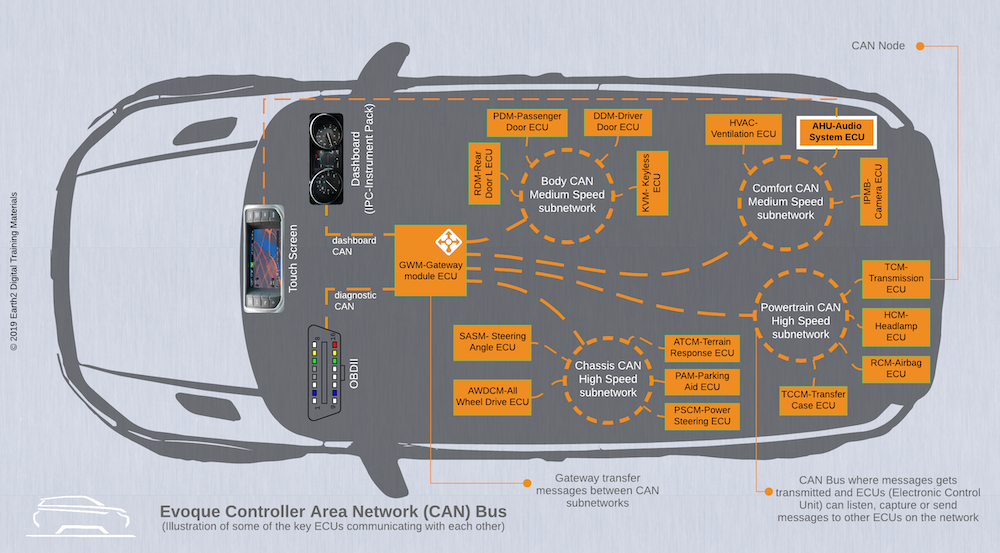
\includegraphics[width=8cm]{CAN_auto.png}
  \caption{Protocollo CAN BUS all'interno di un'autovettura}
  \label{fig:Protocallo CAN-BUS}
\end{figure}
\footnotetext{Presa da: \url{https://farelettronica.it/web/app/uploads/2022/04/02-controller-area-network-ecu-evoque-adam-ali-small.png}}

\paragraph{Il connettore OBD} Molti veicoli sono dotati di un connettore \textbf{OBD-II}, detto anche connettore del collegamento diagnostico (DLC, Diagnostic Link Connector), che comunica con la rete interna del veicolo. Solitamente questo connettore si trova sotto il piantone dello sterzo o nascosto da qualche parte nel cruscotto in una posizione comunque relativamente accessibile.
La tensione a riposo dei cavi CAN è di 2.5V, quando arriva un segnale, sommerà o sottrarrà 1V (3.5V o 1.5V). I fili CAN attraversano il veicolo e collegano le ECU e altri sensori e sono sempre in coppia. Le connessioni CAN high e CAN low sono presenti sui pin 6 e 14 del connettore OBD-II, come illustrato nella figura sottostante \ref{fig:Connettore OBD}. \cite{manualeHacker}


\begin{figure}[h]
  \centering
  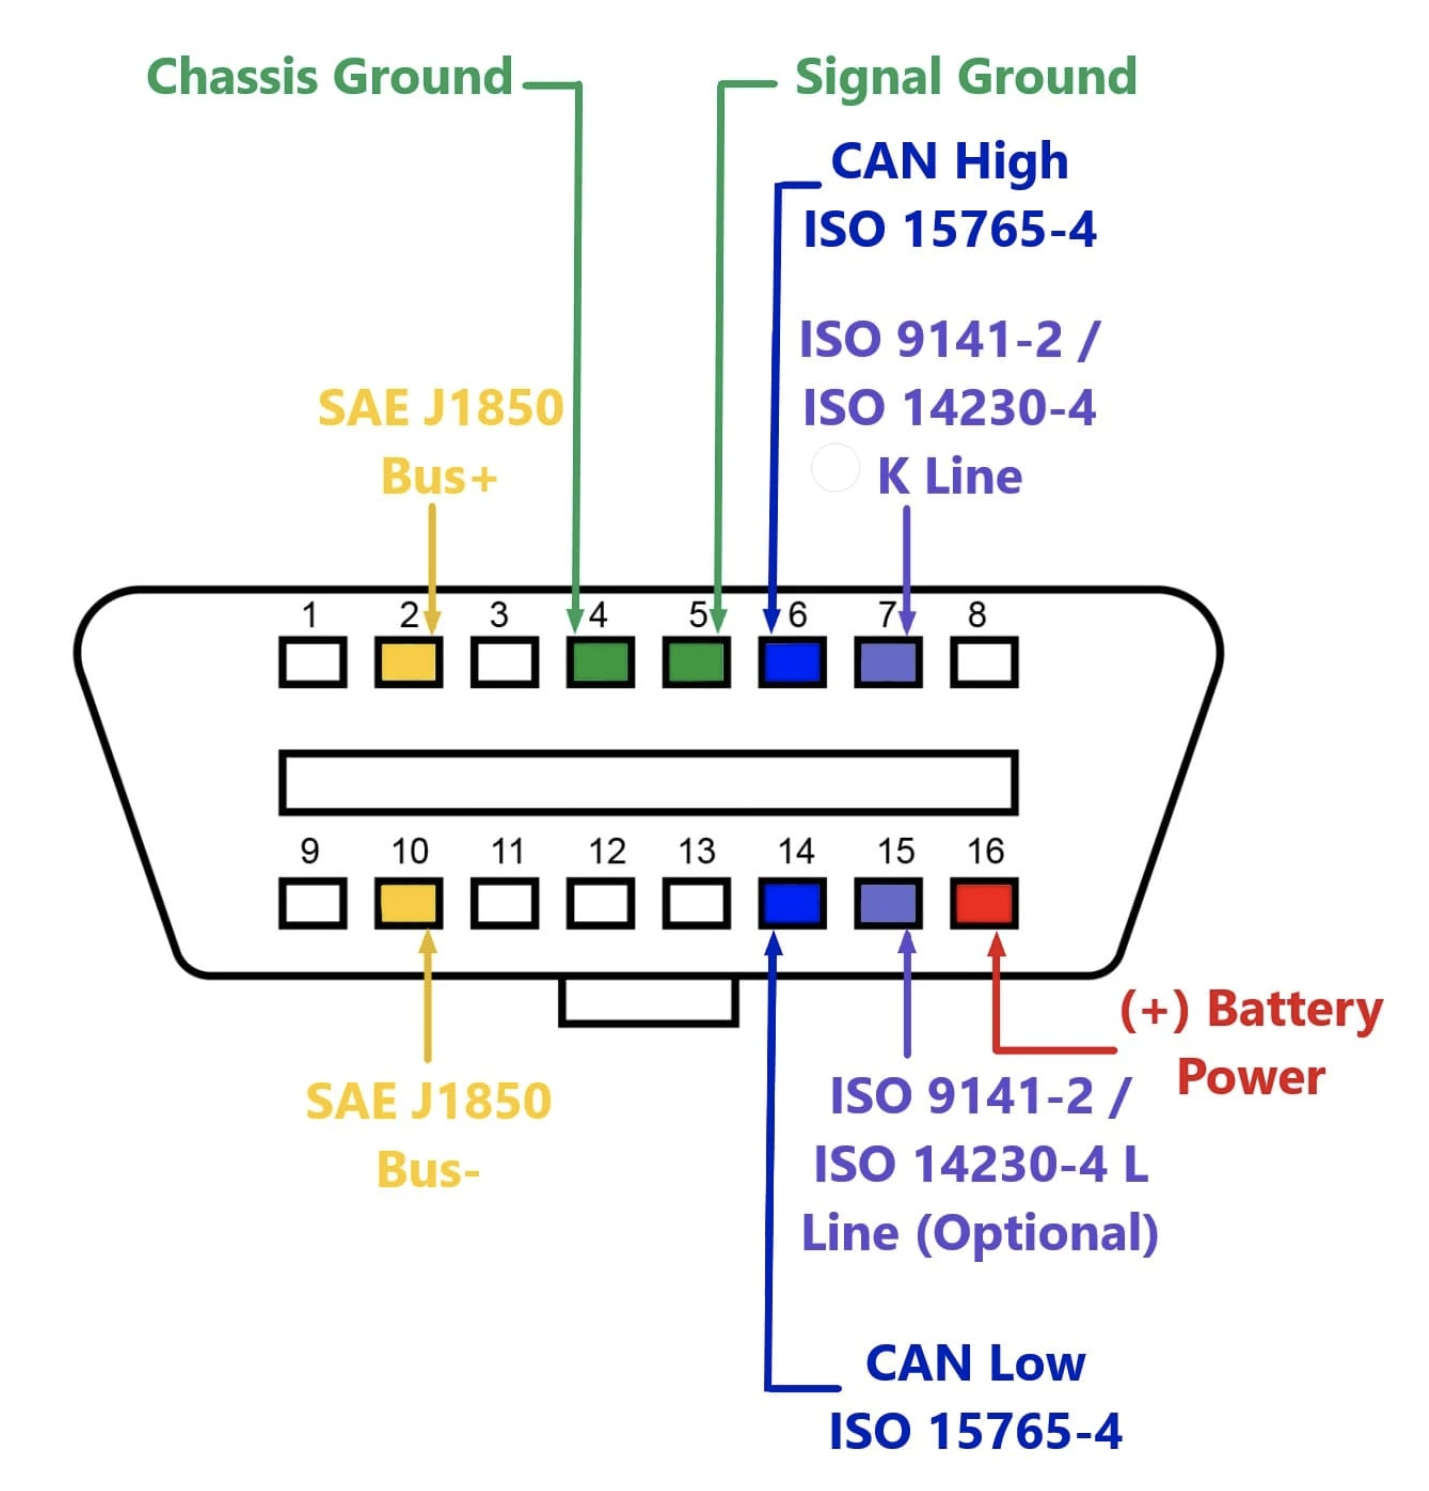
\includegraphics[width=8cm]{Connettore_OBD-II.png}
  \caption{Pin dei cavi CAN sul connettore OBD-II}
  \label{fig:Connettore OBD}
\end{figure}
\footnotetext{Presa da: \url{https://www.flexihub.com/images/upload/flexihub/articles/diagnostics/pinout_explanation.jpg}}

\paragraph{Struttura dei pacchetti del bus CAN}
Vi sono due tipi di pacchetti CAN: 
\textbf{standard} ed \textbf{estesi}. I pacchetti sono come quelli standard, semplicemente hanno uno spazio maggiore per conservare ID. \textbf{Pacchetti standard:} Ogni pacchetto di bus CAN contiene quattro elementi findamentali:
\begin{itemize}
    \item \textbf{L'ID di arbitraggio} (arbitration ID) è un messaggio broadcast che indica l'ID del dispositivo che cerca di comunicare, anche se ogni dispositivo può inviare più ID di arbitraggio. Se sul bus vengono inviati due pacchetti CAN contemporaneamente, vince quello con l'ID di arbitraggio più basso.
    \item \textbf{IDE}, estensione dell'identificatore (Identifier Extension) Questo bit è sempre 0 per i pacchetti CAN standard.
    \item \textbf{DLC}, codice della lunghezza dei dati (Data Length Code) Questa è la dimensione dei dati che varia da 0 a 8 byte.
    \item \textbf{Dati} Questi sono i dati in senso stretto. Le dimensioni massime dei dati veicolati da un pacchetto standard del bus CAN è di 8 byte, ma alcuni sistemi forzano le dimensioni sempre a 8 byte, "imbottendo" il pacchetto.
\end{itemize}

\begin{figure}[h]
  \centering
  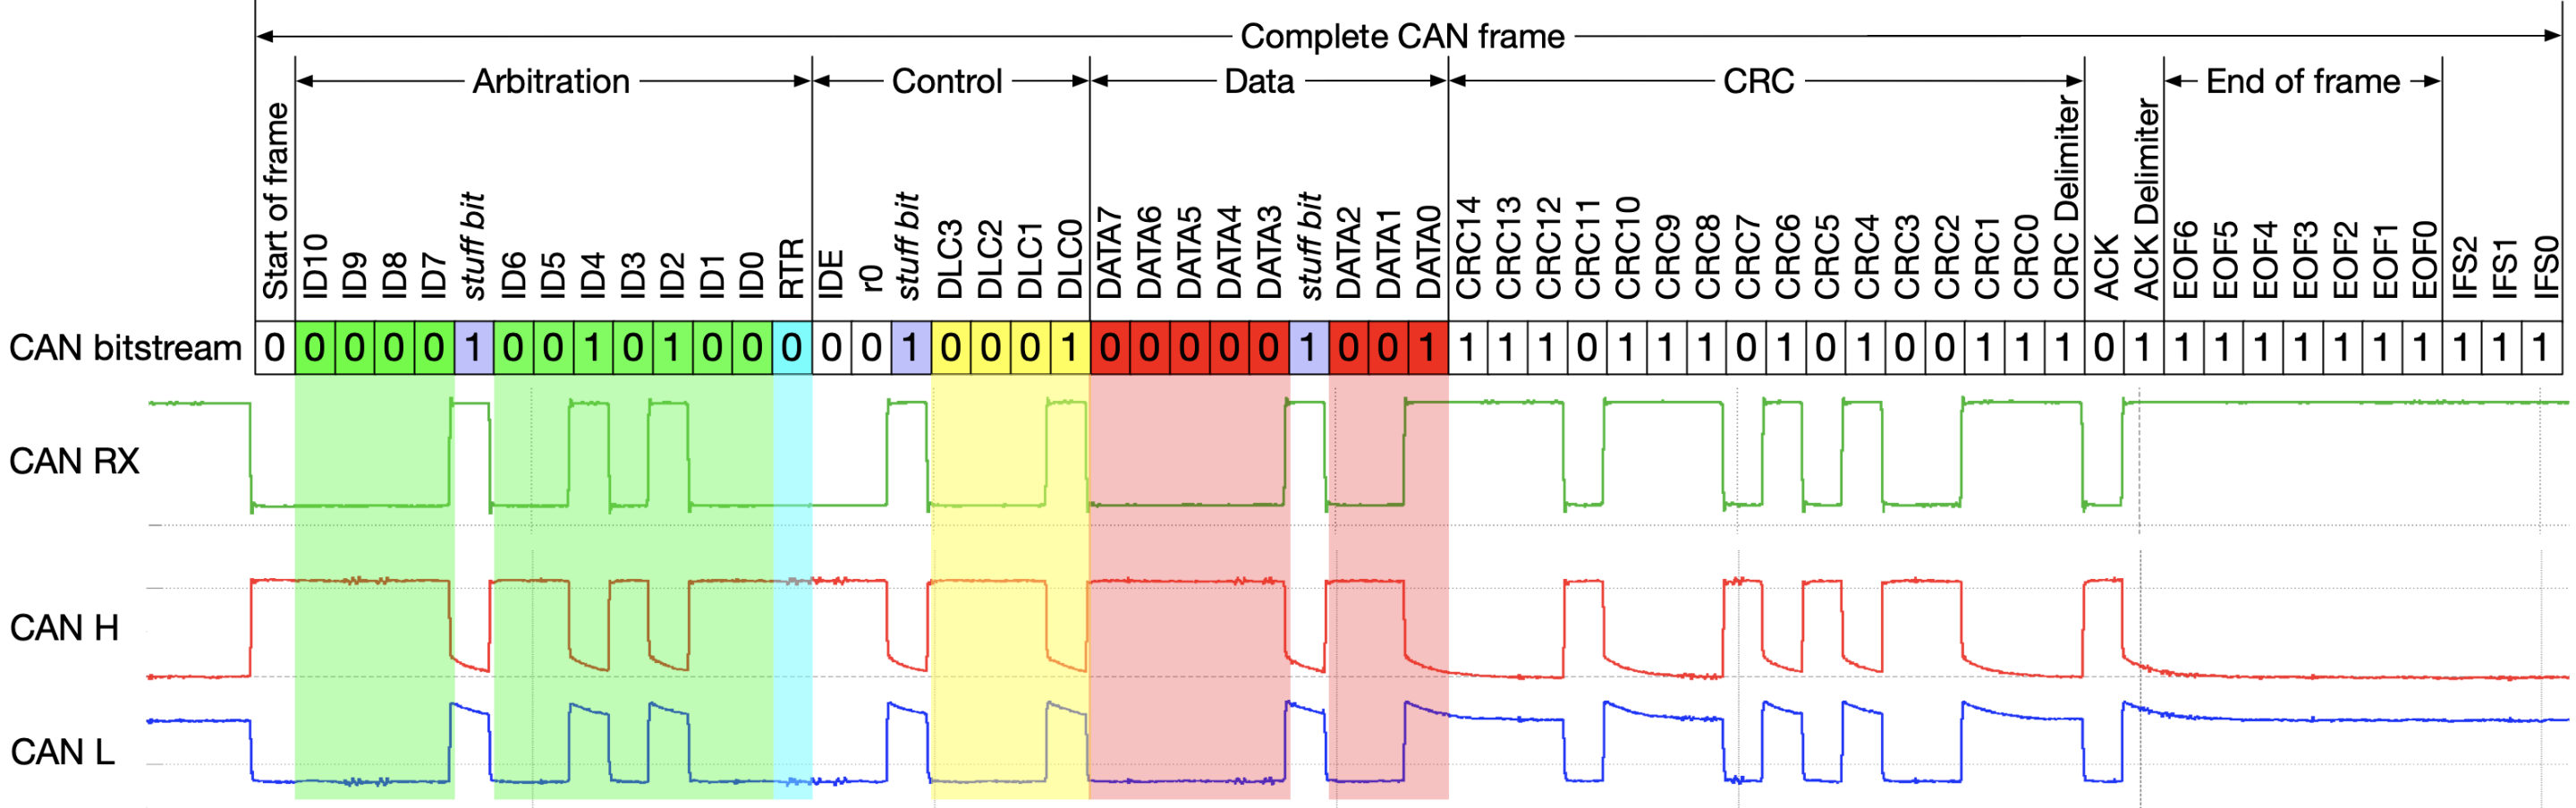
\includegraphics[width=10cm]{FrameCAN.png}
  \caption{Formato dei pacchetti CAN standard}
  \label{fig:pacchettoCAN}
\end{figure}
\footnotetext{Presa da: \url{https://upload.wikimedia.org/wikipedia/commons/5/54/CAN-bus-frame-with-stuff-bit-and-correct-CRC.png}}

Poiché i pacchetti del bus CAN sono di tipo broadcast, tutti i controller sulla stessa rete vedono tutti i pacchetti. I pacchetti non portano con sè informazioni sul controller che li abbia inviati. Poiché qualsiasi dispositivo può vedere e trasmettere pacchetti.

\textbf{Pacchetti estesi:}
I pacchetti estesi sono come quelli standard, tranne che possono essere concatenati fra loro per creare ID più lunghi. I pacchetti estesi sono fatti in modo da adattarsi alla formattazione CAN standard per mantenere la compatibilità a ritroso. Così se un sensore non ha il supporto per i pacchetti estesi, non si guasterà se un altro dispositivo trasmette pacchetti CAN estesi sulla stessa rete. I pacchetti standard e quelli estesi si differenziano anche per l'uso dei flag. Se esaminati i pacchetti estesi in un dump di rete, vedrete che, a differenza di quelli standard, usano un flag \textbf{SSR} (Substitute remote request) anzichè \textbf{RTR} (Remote transmission request), con SSR impostato al valore 1. Avranno anche il campo IDE impostato al valore 1 ed i pacchetti avranno identificatori a 18 bit, che è la seconda parte dell'identificatore standard a 11 bit.

\subsection{OBD scanner - esp32}
Per leggere i messaggi presenti all'interno della rete CAN BUS è necessario di un lettore OBD-II in grado di connettersi con il corrispettivo connettore OBD presente all'interno del veicolo e di trasmettere dati via \textbf{Bluetooth} ad un apparecchio esterno, nel nostro caso l'ESP32. Per leggere e decifrare i messaggi provenienti dalla rete CAN, è stata utilizzata una libreria ELMduino; utile per interfacciare facilmente l'ESP32 con uno scanner OBD-II. Tramite questa libreria è possibile interrogare tutti i PID supportati da OBD-II per raccogliere un'ampia varietà di dati, ad esempio velocità, giri al minuto, temperatura del motore...

\begin{figure}[h]
  \centering
  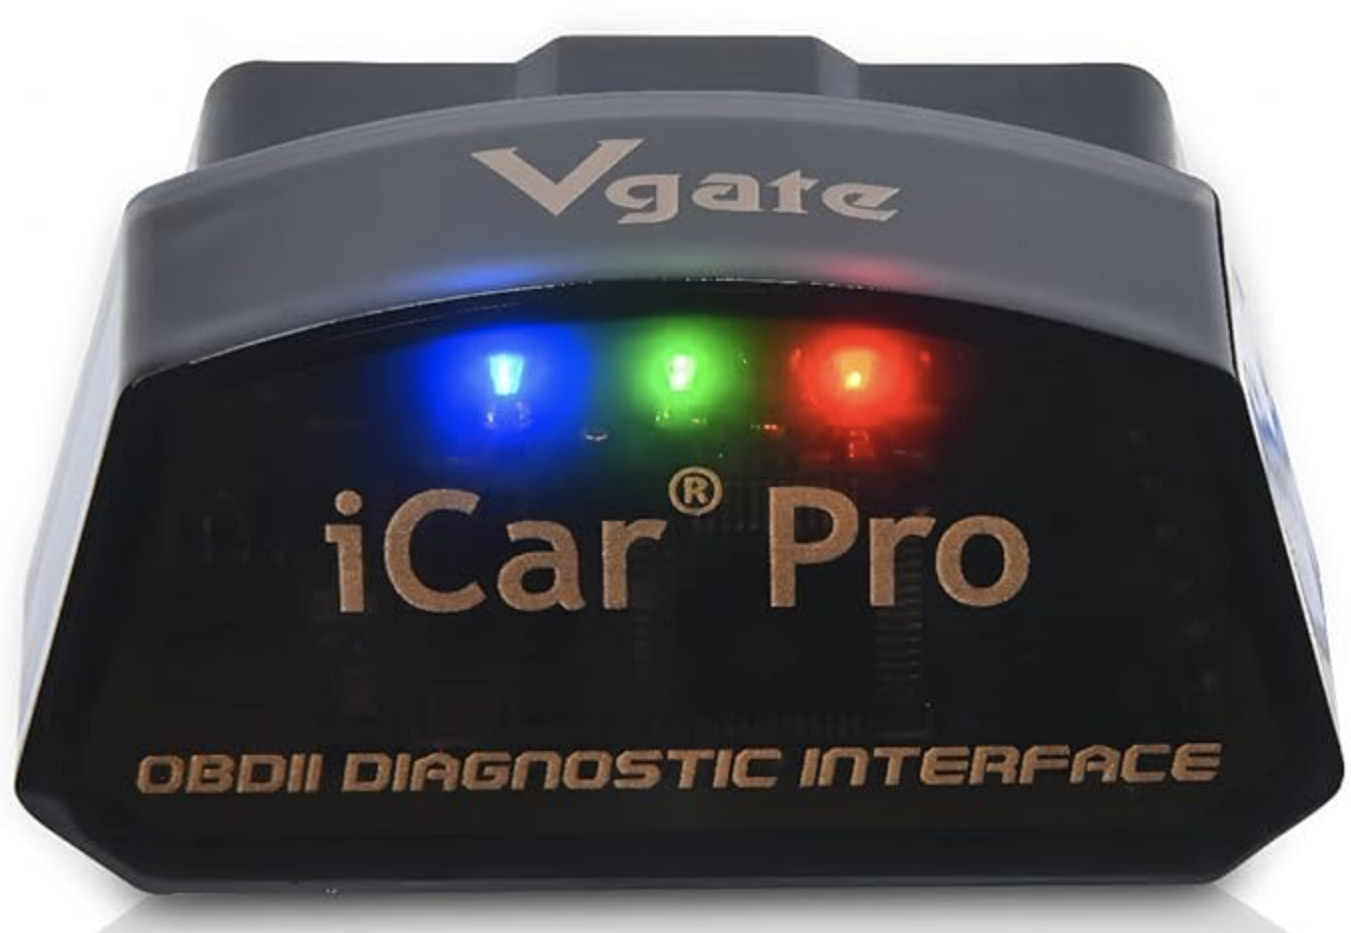
\includegraphics[width=6cm]{LettoreScannerOBD-II.png}
  \caption{Esempio di scanner OBD-II utilizzato per il progetto}
  \label{fig:scannerOBD-II}
\end{figure}
\footnotetext{Presa da: \url{https://m.media-amazon.com/images/I/51crnV3RTbL._AC_SX679_.jpg}}

\subsection{esp32 - server remoto}
Quando la black box rileva la presenza di una connessione Internet, si collega ad un server remoto, il quale è sempre in ascolto, per trasmettere dati relativi al monitoraggio, alla segnalazione di allarmi e sulla profilazione del conducente. 
Nel progetto viene adoperato Netcat, un programma open source a riga di comando di comunicazione remota, utilizzabile sia col protocollo TCP sia col protocollo UDP. Lato server è necessario mettersi in ascolto per ricevere dati al momento di sincronizzazione, dopodichè è possibile redirigere l'output su di un file utilizzato appositamente per la raccolta dati. \cite{Netcat}

\chapter{Risultati ottenuti}
\section{Analisi dei risultati}
Sono state condotte analisi relative alla segnalazione di allarmi e alla profilazione guida. Le prime sono state verificate in modo tale da far sollecitare il task relativo al rilevamento della situazione anomala e verificare che venga esibito sul display lcd il relativo avviso di pericolo, o la relativa notofica di comportamento errato, e verificato ulteriormente che al server fossero arrivate le opportune notifiche. 

\begin{figure}[h]
  \centering
  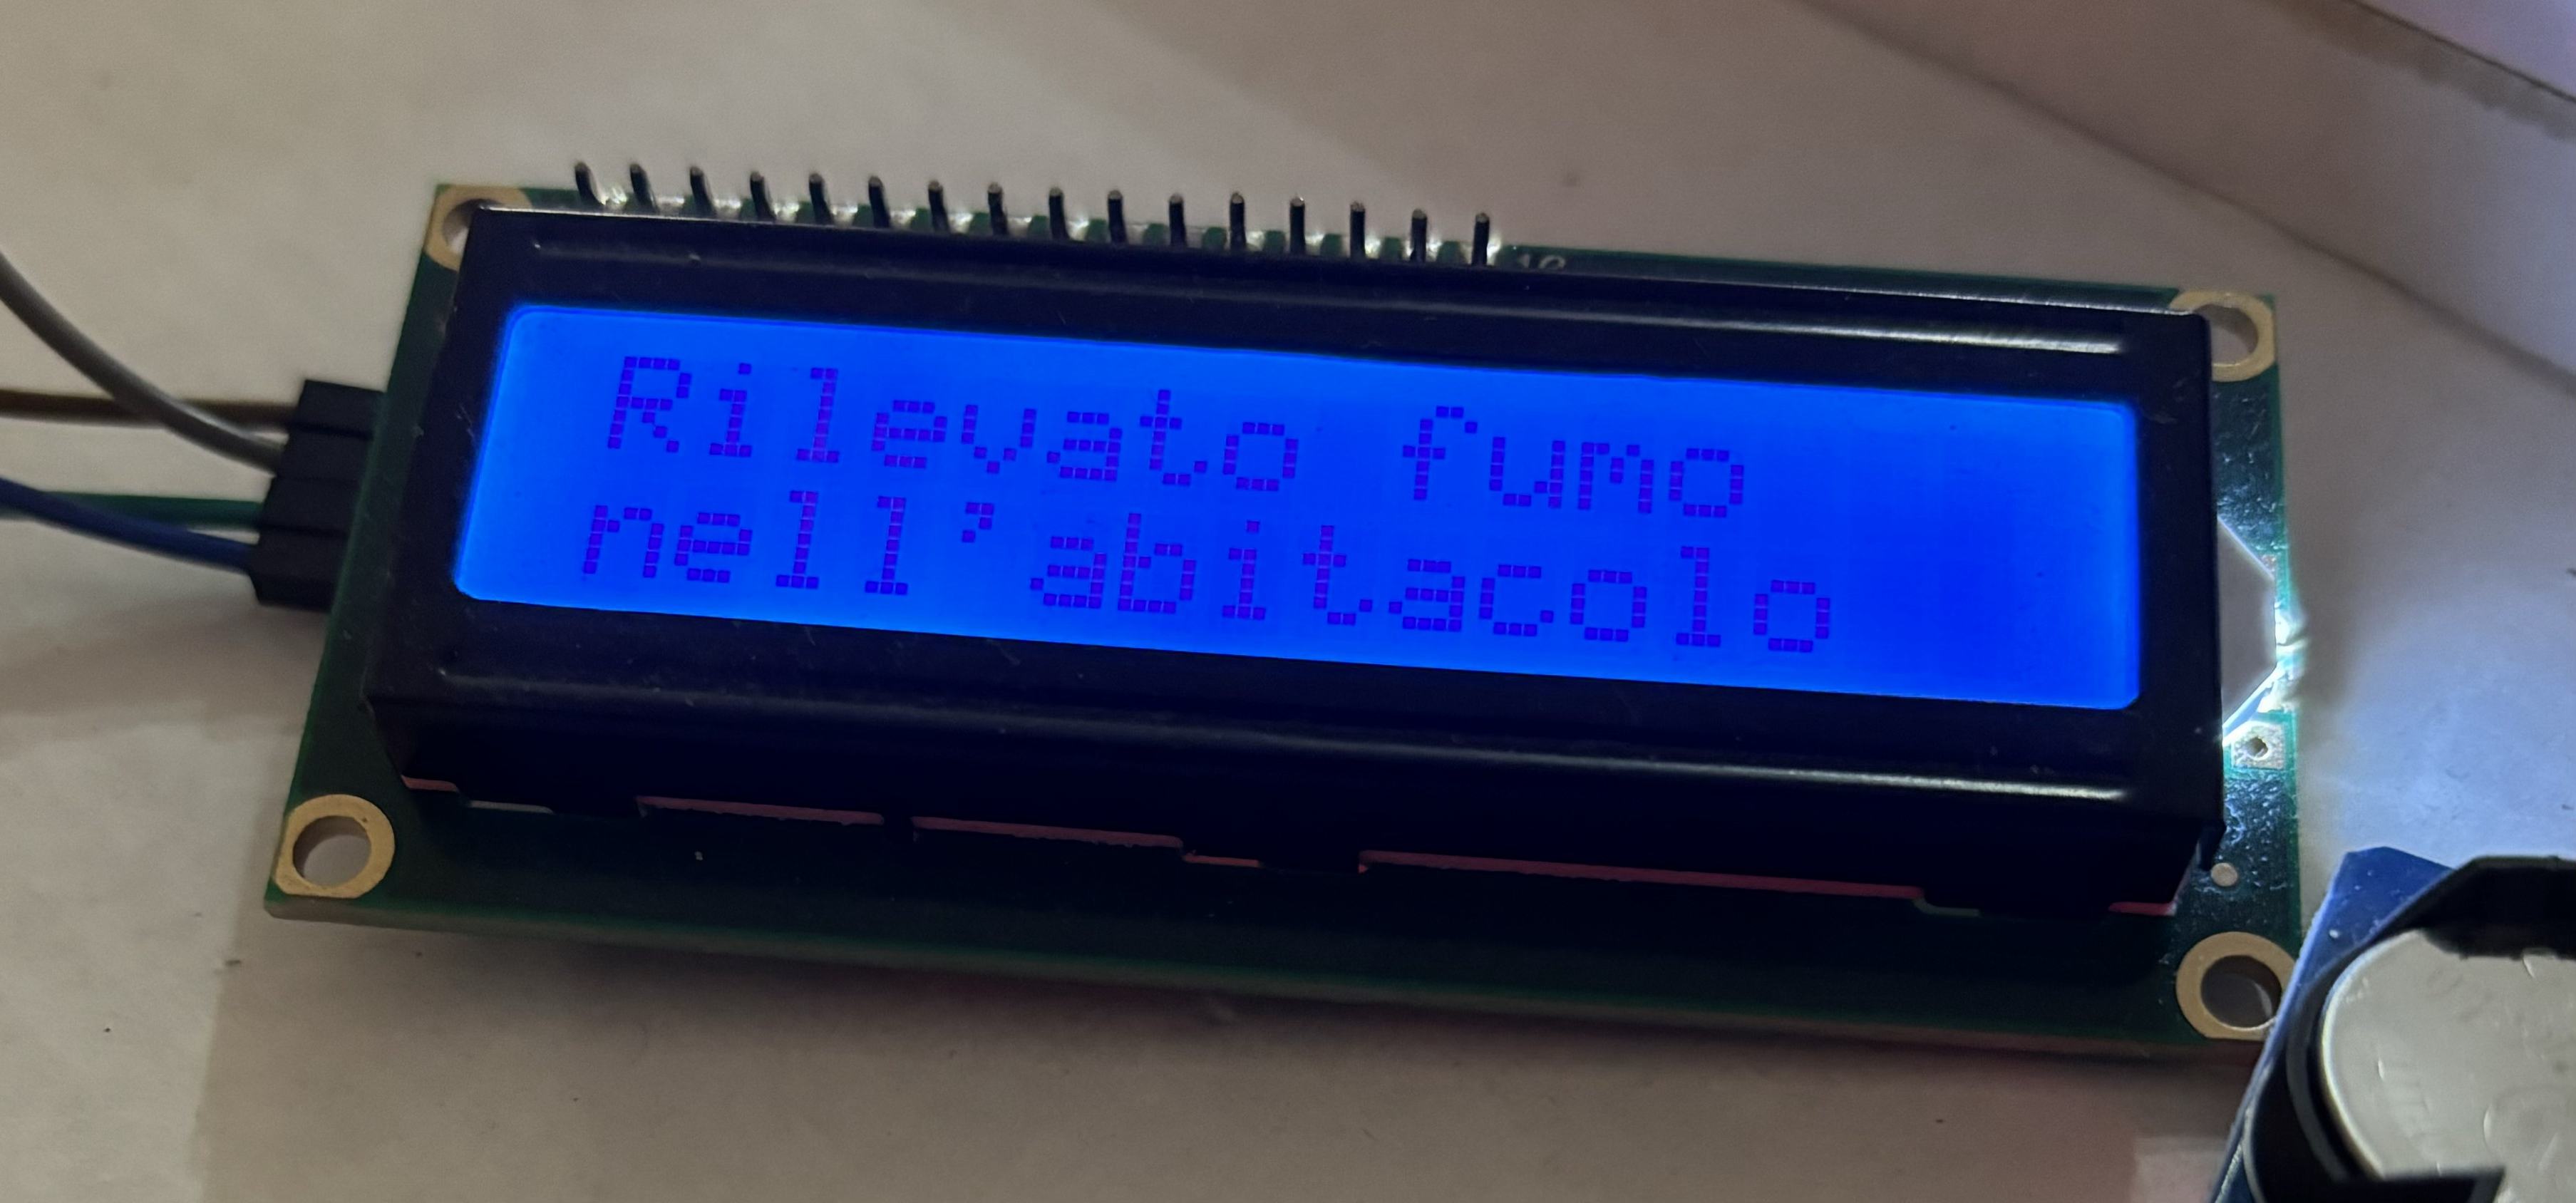
\includegraphics[width=8cm]{fumoLCD.png}
  \caption{Display presente sulla black box che notifica al guidatore il fatto di aver rilevato una presenza di fumo nell'abitacolo}
  \label{fig:fumoLCD}
\end{figure}

\begin{figure}[h]
  \centering
  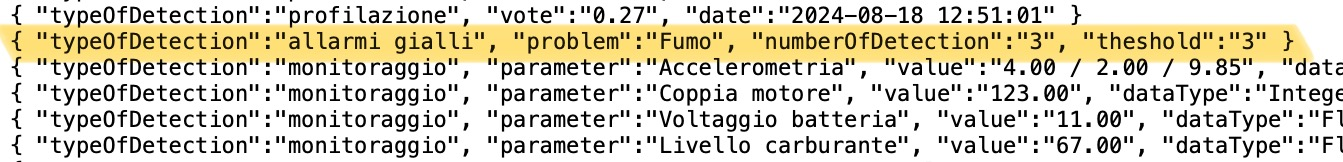
\includegraphics[width=14cm]{fumoServer.jpg}
  \caption{Esempio di notifica ricevuta dal server remoto a seguito aver rilevato più volte la presenza di fumo nell'abitacolo}
  \label{fig:fumoServer}
\end{figure}

Per quanto riguarda la profilazione guida sono state simulate 3 guide da 20 min circa ciascuna. Per ogni guida sono stati modificati i parametri relativi alla profilazione del guidatore così da poter distinguere ciascuna di esse in 3 diverse categorie: guida \textbf{brusca, intermedia e moderata}. I parametri che sono stati simulati sono: accelerometria lungo i due assi x e y, i giri motore (rpm), la velocità del veicolo (kph), la posizione della valvola a farfalla e il carico motore. 

\begin{table}[h!]
  \centering 
  \begin{adjustbox}{max width=\textwidth}
    \begin{tabular}{|c|c|c|c|c|c|c|c|}
      \hline
      \textbf{Stile guida} & \textbf{acc. asse x} & \textbf{acc. asse y} & \textbf{rpm} & \textbf{kph} & \textbf{throttle} & \textbf{engine load} & \textbf{voto} \\
      \hline
      Spericolato & $[4,9] \ \text{m/s}^2$ & $[4,9] \ \text{m/s}^2$ & $[3000,4000] \ \text{giri/min}$ & $[0,130] \ \text{km/h}$ & $[40,90] \%$ & $[30,70] \%$  & 0.695\\
      \hline
      Intermedio & $[2,7] \ \text{m/s}^2$ & $[2,7] \ \text{m/s}^2$ & $[2000,3000] \ \text{giri/min}$ & $[0,130] \ \text{km/h}$ & $[30,70] \%$ & $[20,60] \%$  & 0.428\\
      \hline
      Moderato & $[0,5] \ \text{m/s}^2$ & $[0,5] \ \text{m/s}^2$ & $[1500,2500] \ \text{giri/min}$ & $[0,130] \ \text{km/h}$ & $[20,50] \%$ & $[10,50] \%$  & 0.328\\
      \hline
    \end{tabular}
  \end{adjustbox}
  \caption{Tabella rappresentante i range dei valori dei parametri utili alla profilazione del conducente, rappresentanti diversi stili di guida con relativa attribuzione del voto.}
  \label{tab:stili_di_guida}
\end{table}

Per concludere questo paragrafo di seguito saranno presentati i dati di monitoraggio, segnalazione di allarmi e profilazione guida ricevuti dal server a seguito di una sincronizzazione:

\begin{figure}[h]
  \centering
  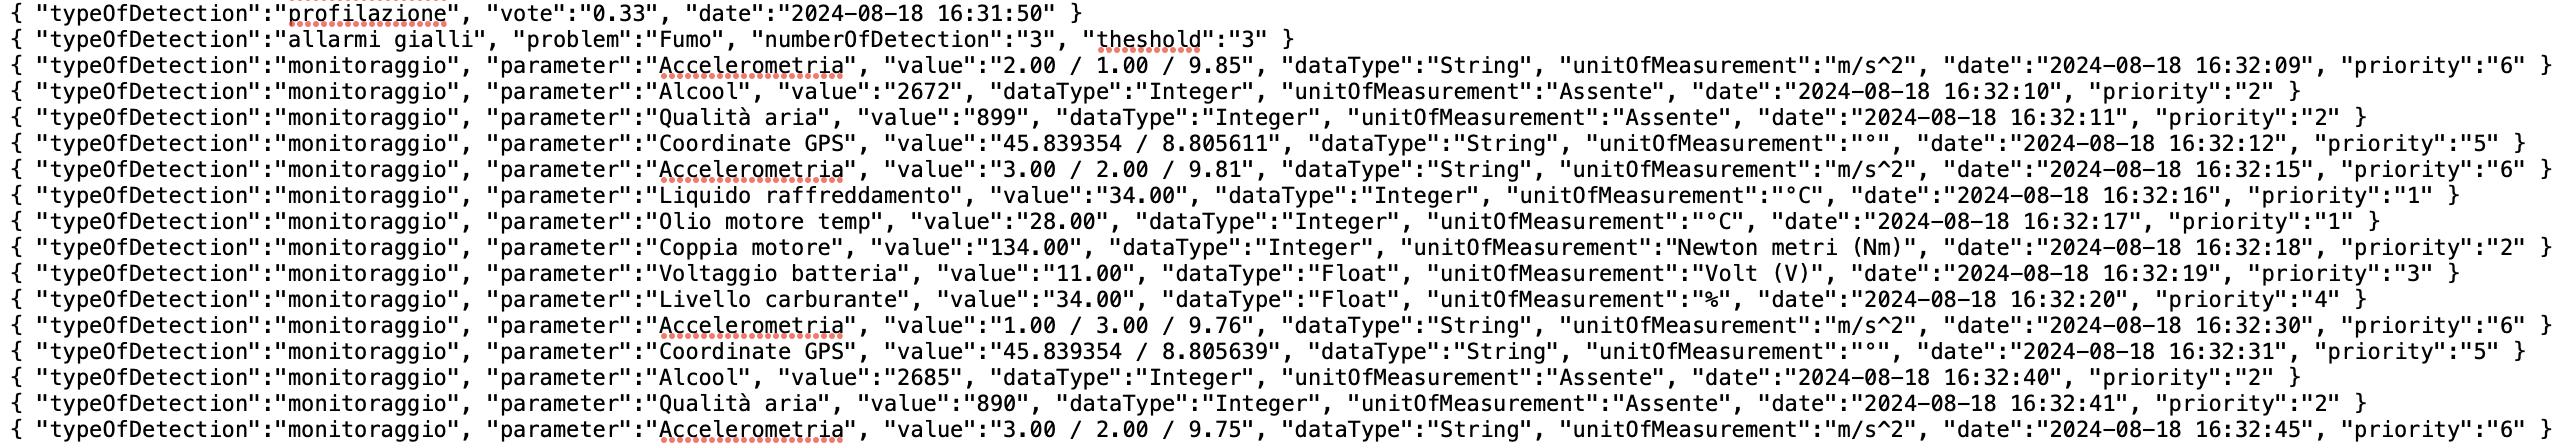
\includegraphics[width=16cm]{datiServer.png}
  \caption{Ricezione dati lato server}
  \label{fig:datiServer}
\end{figure}

\section{Comportamenti non implementati}
Alcuni comportamenti relativi alla segnalazione di allarmi critici e non non sono stati implementati. Questi riguardano la gestione degli allarmi relativi al \textbf{consumo anomalo di carburante} e alla \textbf{distanza di frenata anomala} per quanto riguarda gli allarmi critici, il \textbf{rilevamento della presenza di fumo} per quanto riguarda invece gli allarmi meno critici. Quest'ultima funzionalità è facilmente implementabile con l'installazione di un sensore apposito che rileva la presenza di fumo nell'ambiente che lo circonda; l'implementazione delle prime due funzionalità è stata volutamente non implementata data la complessa natura dei due problemi, che richiedono uno studio complesso e approfondito. Questi aspetti rimangono importanti per sviluppi futuri e rappresentano punti chiave per migliorare ulteriormente il sistema.

Un altro componente non installato nel sistema attuale è il \textbf{modulo GSM con relativa antenna}, che permette la comunicazione con il server remoto della centrale operativa indipendentemente dalla disponibilità di una rete WiFi.
L'installazione del modulo GSM può essere facilmente eseguito seguendo due approcci: 

\begin{itemize}
    \item \textbf{Modulo separato}: un modulo GSM con relativa antenna può essere facilmente aggiunto al sistema esistente. Questi moduli sono ampiamente disponibili e possono essere integrati con l'ESP32 attraverso interfacce standard, vedi figura  \ref{fig:modulo_gsm}.
    \item \textbf{Modulo integrato}: esistono versioni dell'ESP32 che includono un modulo GSM integrato, semplificando ulteriormente l'implementazione di questa funzionalità senza la necessità di componenti aggiuntivi, vedi figura \ref{fig:esp32_gsm}.
\end{itemize}

\begin{figure}[h]
  \centering
  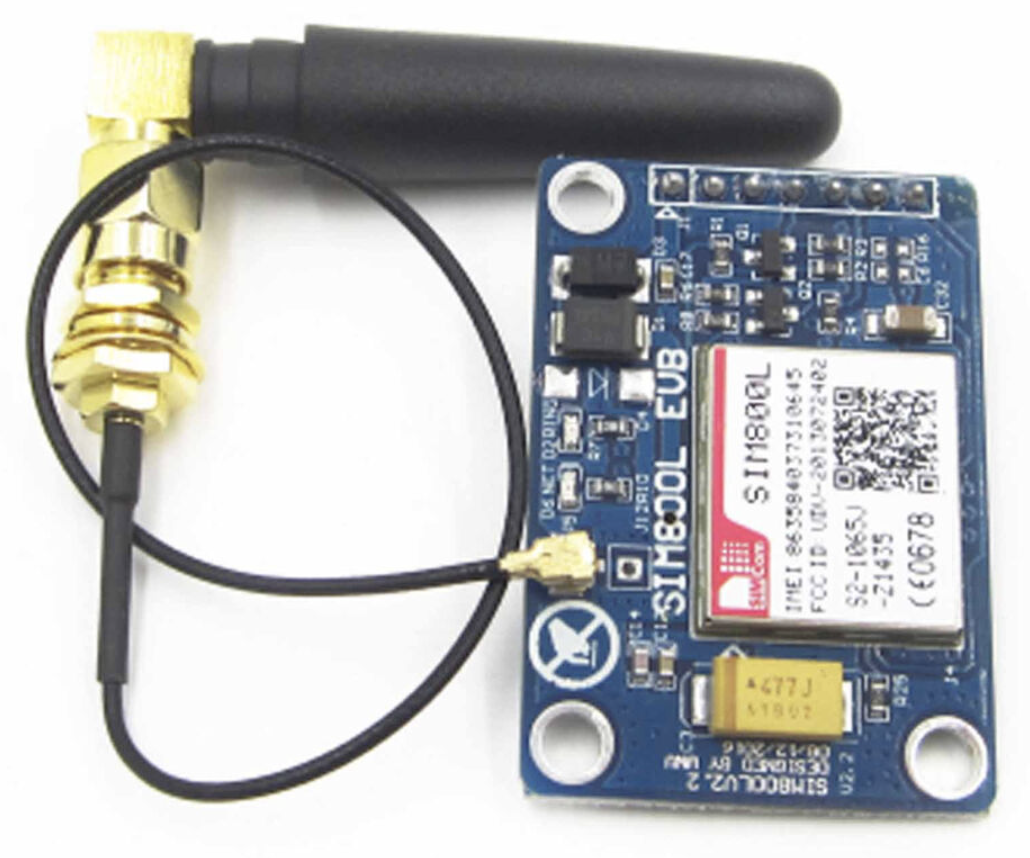
\includegraphics[width=6cm]{gsm_module.png}
  \caption{Modulo GSM da integrare}
  \label{fig:modulo_gsm}
\end{figure}
\footnotetext{Presa da: \url{https://i.ebayimg.com/images/g/~dEAAOSwmwdhZkO7/s-l1200.jpg}}

\begin{figure}[h]
  \centering
  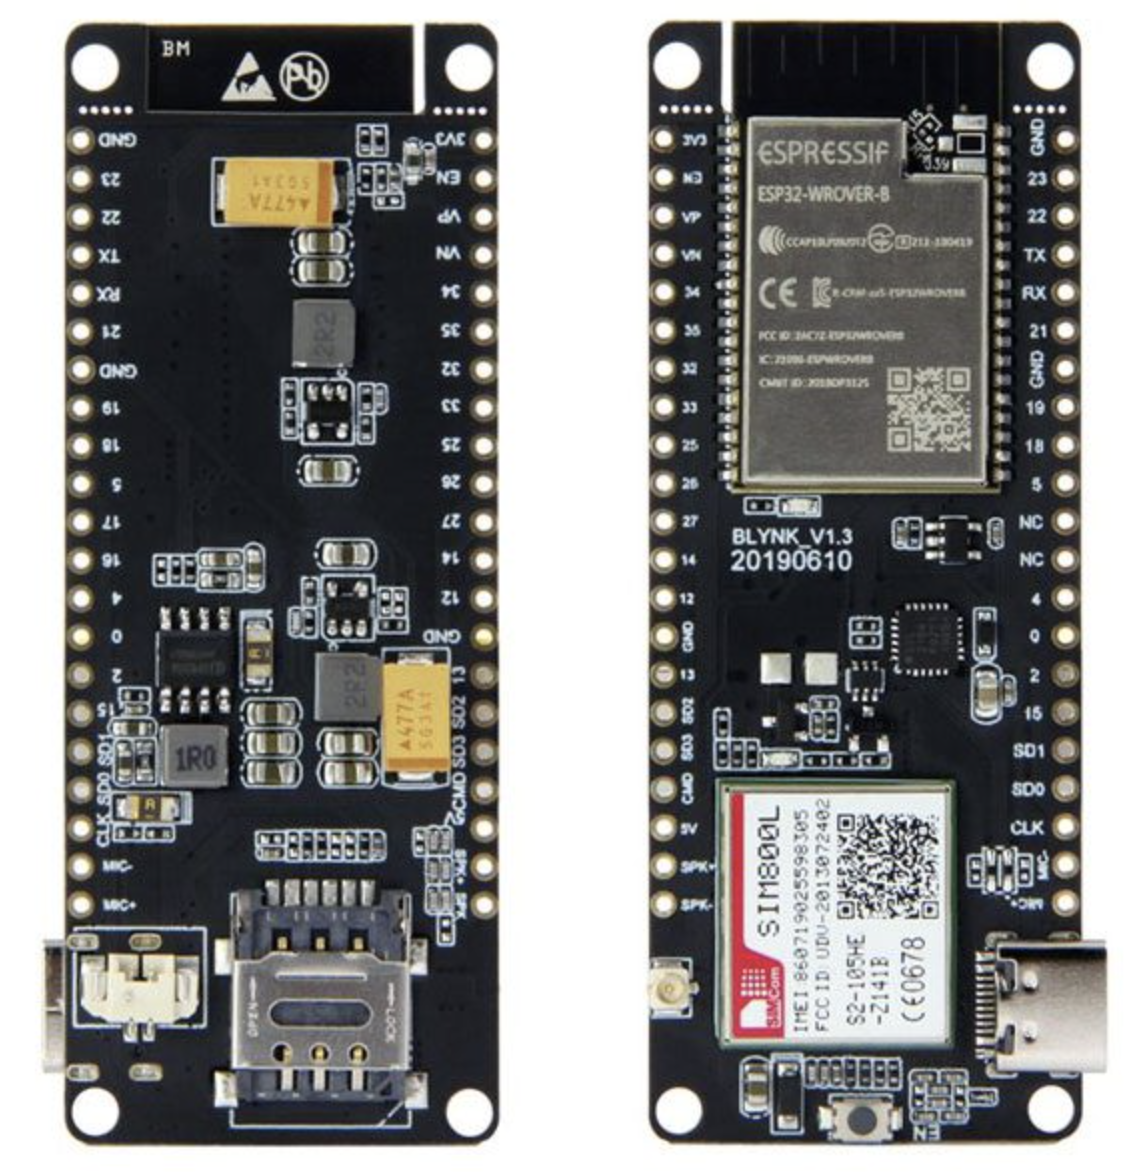
\includegraphics[width=6cm]{esp32_gsm.png}
  \caption{ESP32 SIM800L}
  \label{fig:esp32_gsm}
\end{figure}
\footnotetext{Presa da: \url{https://futuranet.it/wp-content/uploads/2021/02/1606-HR1761.jpg}}

\chapter{Conclusioni}
\section{Problemi aperti}
\paragraph{Problema di decremento dello spazio di storage}
Nel sistema black-box sono presenti due task che hanno il compito di ripulire la memoria del microcontrollore, vedi paragrafo \ref{sec:Sincronizzazione}, uno di routine che elimina i record già sincronizzati ed uno che elimina i record se viene superata una soglia massima di occupazione del filesystem (90\%), eliminando la metà dei record di monitoraggio meno recenti. Il problema riscontrato risale a quest'ultimo task. Lo spazio di storage man mano che vengono memorizzati record aumenta in modo corretto, tuttavia a seguito delle operazioni di pulizia dei record effettuate dal task di routine che rimuove dalla tabella di monitoraggio i record già sincronizzati, lo spazio di storage non diminuisce come previsto. Tale problema persiste anche dopo aver tentato di utilizzare un particolare comando \textbf{VACUUM}, che solitamente dovrebbe riorganizzare il database e liberare lo spazio inutilizzato. 
Tale task di pulizia, che riguarda il monitoraggio della capacità di memoria del filesystem e l'eliminazione dei record meno recenti, non è stato implementato nel codice.

\section{Sviluppi futuri}
\subsection{Memoria}
Negli sviluppi futuri del progretto, un'area di miglioramento fondamentale è l'integrazione di una memoria esterna con la board. Questa aggiunta apporterà significativi vantaggi operativi e funzionali, suddivisibili in due principali categorie: l'aumento dello spazio di storage per il monitoraggio del veicolo e la capacità di caricare e utilizzare mappe stradali per verificare il rispetto dei limiti di velocità.

\begin{figure}[h]
  \centering
  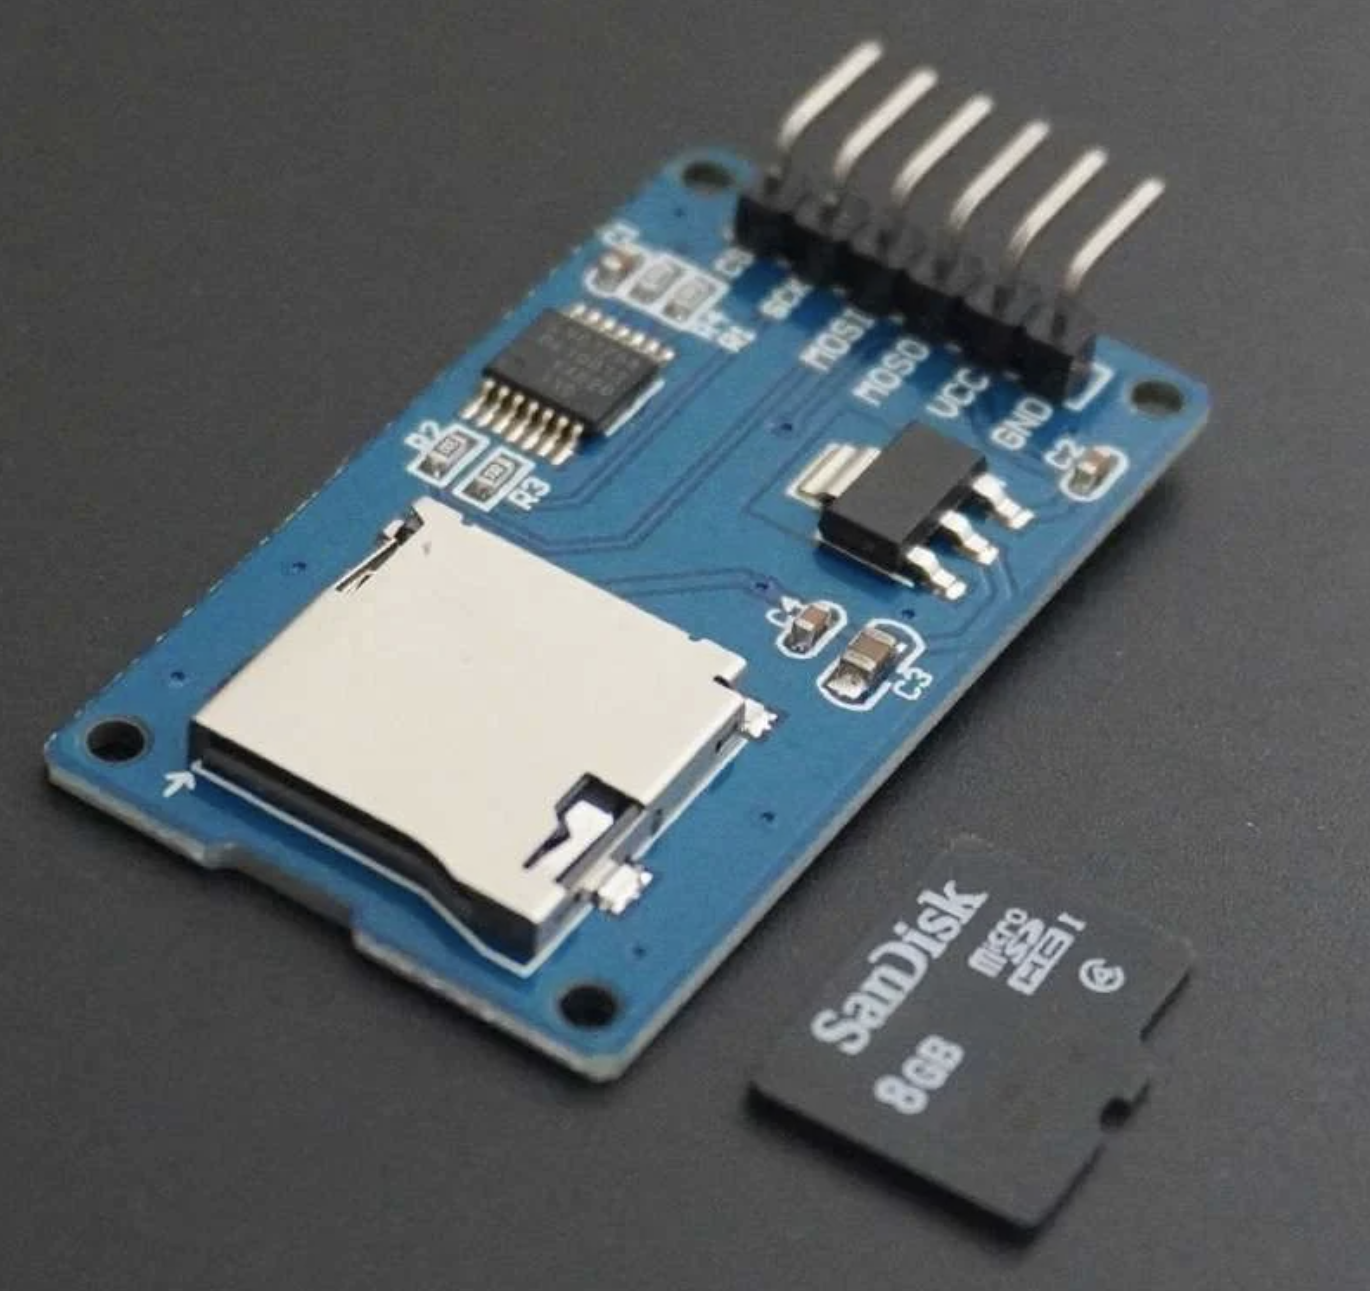
\includegraphics[width=8cm]{MicroSD.png}
  \caption{Micro SD card}
  \label{fig:MicroSD}
\end{figure}
\footnotetext{Presa da: \url{https://www.electronicwings.com/storage/PlatformSection/TopicContent/452/description/MicroSD.jpg}}

\paragraph{Maggiore spazio di storage per il monitoraggio del veicolo} 
Uno dei limiti attuali dell'ESP32 è la sua capacità di storage relativamente limitata (4MB), che può rappresentare un ostacolo nel contesto del monitoraggio continuo dei dati del veicolo. L'integrazione di una memoria esterna, come una scheda microSD o modulo di memoria flash, può aumentare notevolmente la quantità di dati che possono essere registrati e memorizzati. Questo incremento di capacità di storage consente di:

\begin{itemize}
    \item \textbf{Monitoraggio continuo}: registrare dati continuamente per periodi più estesi senza preoccuparsi di esaurire lo spazio disponibile.
    \item \textbf{Sincronizzazione rara con il server remoto}: ridurre la necessità di sincronizzare frequentemente i dati raccolti con un server centrale. I dati possono essere raccolti e conservati localmente per lunghi periodi e sincronizzati solo quando una rete WiFi stabile è disponibile. Attualmente il sistema prevede la sincronizzazione una volta al giorno, anche se è possibile sincronizzare più raramente.
\end{itemize}

\paragraph{Caricamento di mappe per il rispetto dei limiti di velocità} 
Un'altra funzionalità utile per la profilazione che potrebbe essere implementata con l'aggiunta di una memoria esterna è la possibilità di caricare e gestire mappe stradali. Questa capacità può essere adoperata per monitorare il rispetto dei limiti di velocità del veicolo in diverse aree geografiche. I vantaggi includono:

\begin{itemize}
    \item \textbf{Verifica del rispetto dei limiti di velocità}: Utilizzando mappe che includono informazioni sui limiti di velocità in zone urbane, extraurbane. e autostradali, il sistema può monitorare in tempo reale se il veicolo rispetta i limiti imposti in ogni tratto stradale.
    \item \textbf{Sicurezza stradale}: aumentare la sicurezza stradale, informando il conducente in caso di superamento dei limiti di velocità. 
\end{itemize}

\subsection{Profilazione conducente lato server remoto} 
Per concludere il nostro studio possiamo affiancare alla capacità della board di valutazione del guidatore, tecniche di Machine Learning relative sia all'apprendimento supervisionato che non supervisionato, consentendoci di esaminare più approfonditamente la natura della nostra flotta. In questo contesto, ci concentreremo su due principali tecniche di Machine Learning: la \textbf{classificazione} e il \textbf{clustering}. La classificazioneci permette di assegnare ai guidatori delle etichette, come ad esempio 'prudente' piuttosto che 'negligente', in base ai loro comportamenti al volante, mentre il clustering ci consente di raggruppare i guidatori in base a similitudini nel comportamento di guida. Esploreremo queste tecniche nel dettaglio, evidenziando le loro applicazioni specifiche e i benefici che possono apportare all'analisi e alla gestione dell'autonoleggio. \cite{wiki:Apprendimento_automatico}

\vspace{0.5cm}
\paragraph{Machine Learning nell'analisi dei guidatori: applicazioni nel nostro contesto}
Una volta processati i dati relativi all'analisi di profilazione del guidatore, essi possono essere inviati ad un server remoto. Dopodichè è possibile usare varie tecniche di machine learning di apprendimento supervisionato ad esempio la \textbf{classificazione} o di apprendimento non supervisionato ad esempio il \textbf{clustering}, per assegnare ai clienti dell'autonoleggio una certa etichetta di classificazione o raggrupparli in cluster in modo tale da poter osservare un generale comportamento della flotta.

\paragraph{Apprendimento supervisionato}
La \textbf{classificazione} è una tecnica di apprendimento supervisionato, l'obiettivo è quello di predire la classe di appartenenza di un'istanza di input in un insieme discreto di classi; ad esempio, classificare se una mail è spam o non, se un paziente è soggetto a diabete o meno e molti altri esempi. Nel nostro caso di studio vorremmo poter classificare i clienti come guidatori prudenti o negligenti in base ai valori di valutazione studiati durante l'analisi di profilazione fatta precedentemente \ref{sec:AnalisiProfilazione}. Questa tecnica di ML prevede la suddivisione dei dati in due insiemi distinti: un insieme di addestramento e un insieme di test. L'insieme di addestramento viene adoperato per addestrare il modello, mentre l'insieme di test viene utilizzato per valutarne le prestazioni su dati non visti. Per addestrare un modello di apprendimento supervisionato, vengono utilizzati diversi algoritmi che si differenziano per tipo di problema e per tipo di dati. Alcuni esempi di algoritmi comuni includono Support Vector Machine (SVM), Random Forest, Decision Tree, Neural Networks e Regressione Lineare. Dopo l'addestramento, il modello viene valutato utilizzando l'insieme di test. Una volta soddisfatti delle prestazioni del modello, esso può essere pubblicato, implementato in un'applicazione o integrato in un sistema più ampio per fare previsioni su nuovi dati \cite{muhammad2015supervised}. Di seguito un esempio di classificazione binaria: 

\begin{figure}[h] \centering
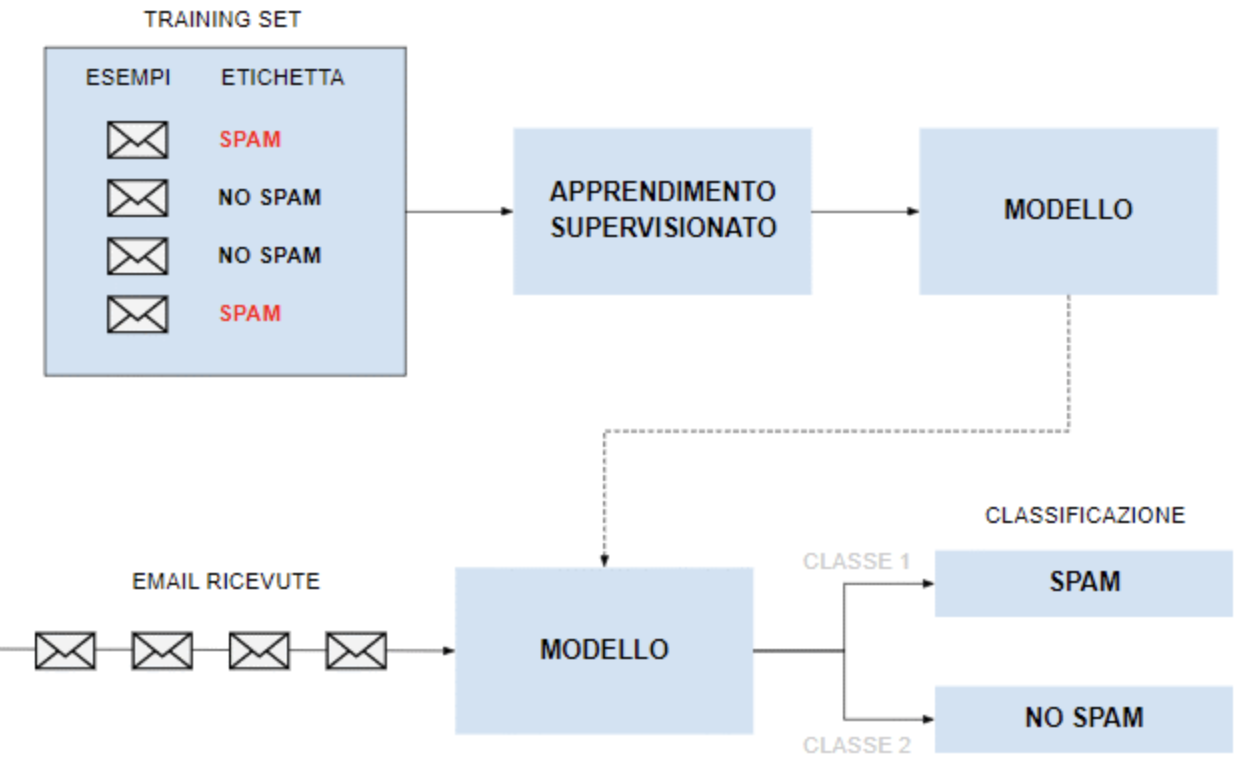
\includegraphics[width=10cm]{Classificazione.png}
\caption{Esempio di classificazione binaria che stabilisce se una email è spam o no\protect\footnotemark}
\label{fig:Classificazione binaria}
\end{figure}
\footnotetext{Presa da: \url{https://www.andreaminini.com/data/andreaminini/apprendimento-supervisionato-esempio-1.gif}}
Se nel nostro studio si volesse classificare il guidatore in più classi, prudente, moderato, negligente ad esempio, con lo scopo di stipulare un contratto assicurativo in base allo stile di guida, esiste la classificazione multiclasse dove sono presenti più di due classi possibili tra cui scegliere e dove ogni istanza da classificare può appartenere ad una sola classe tra le possibili.

\paragraph{Apprendimento non supervisionato}
Il \textbf{clustering} è una tecnica di apprendimento non supervisionato il cui scopo è quello di raggruppare un insieme di oggetti in cluster; gli oggetti dovranno avere un'alta similarità intra-cluster e una bassa inter-cluster. E' una tecnica molto complessa dato che i vari algoritmi imparano osservando i dati e non tramite degli esempi. Grazie a questa tecnica è possibile visualizzare il comportamento dei guidatori della flotta. L'ideale utopico sarebbe quello di avere cluster il cui valore medio che li rappresenta contenga valori di valutazione, quelli citati nella sezione relativa alla profilazione, ragionevoli o che non si discostino troppo dai valori attesi del guidatore prudente.

\vspace{0.5cm}
Di seguito vengono suggerite alcune tecniche che potrebbero essere utilizzate per clusterizzare i propri clienti \cite{popat2014review}: 

\begin{itemize}
    \item Clustering partizionale
    \item Clustering gerarchico
    \item Clustering basato sulla densità
\end{itemize}

\paragraph{Clustering partizionale} 
Il clustering partizionale è la tecnica più comunemente utilizzata tra gli algoritmi di clusterizzazione. Questi algoritmi lavorano per minimizzare un determinato criterio di clustering, spostando iterativamente i punti dati tra i cluster fino a raggiungere una partizione ottimale. Questo approccio suddivide gli oggetti in K partizioni, ognuna delle quali rappresenta un cluster. La suddivisione avviene in base ad una specifica funzione obiettivo. I cluster vengono formati per ottimizzare un criterio di partizionamento definito, come una funzione di dissimilarità basata sulla distanza, in modo che gli oggetti all'interno di un cluster siano considerati "simili", mentre quelli in cluster diversi siano considerati "dissimili". I metodi di clustering partizionale sono particolarmente adatti per applicazioni in cui è richiesto un numero predefinito di cluster, alcuni esempi di algoritmi di clustering includono K-means, PAM (Partition Around Medoids) e Clara.

\begin{figure}[h] \centering
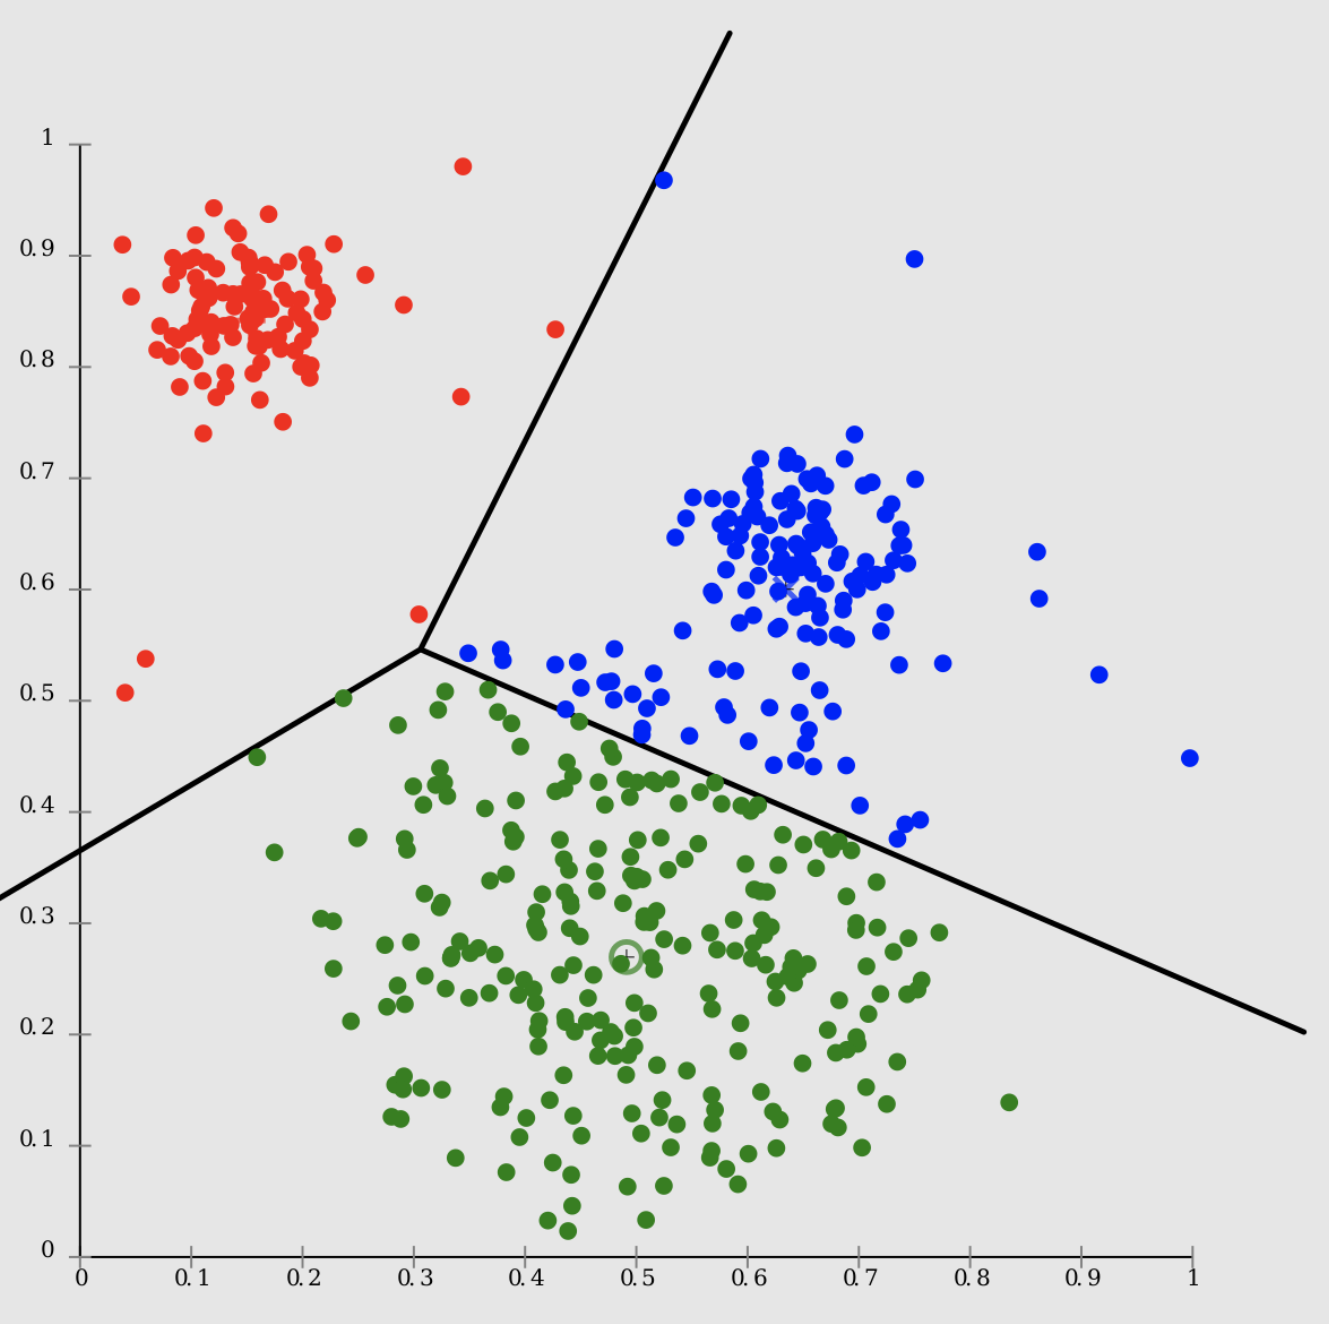
\includegraphics[width=8cm]{C_Partizionale.png}
\caption{K-means usato per la classificazione di 3 partizioni\protect\footnotemark}
\label{fig:esempio k-means}
\end{figure}
\footnotetext{Presa da: \url{https://upload.wikimedia.org/wikipedia/commons/thumb/e/e5/KMeans-Gaussian-data.svg/1280px-KMeans-Gaussian-data.svg.png}}

\paragraph{Clustering gerarchico} 
Gli algoritmi di clustering gerarchico dividono o uniscono un dataset in una sequenza di partizioni nidificate. La gerarchia delle partizioni nidificate può essere agglomerativa (bottum-up) o divisiva (top-down). Nella metodologia agglomerativa, il clustering inizia con ogni singolo oggetto in un singolo cluster e continua a raggruppare le coppie di cluster più vicine fino a quando tutti gli oggetti sono insieme in un unico cluster. Il clustering gerarchico divisivo, d'altra parte, inizia con tutti gli oggetti in un singolo cluster e continua a dividere i cluster più grandi in cluster più piccoli fino a quando tutti gli oggetti sono separati in cluste unitari. Entrambi i metodi gerarchici possono essere rappresentati naturalmente da un dendogramma, che illustra la struttura dei cluster. Esempi di questi algoritmi sono Rock, Birch (Balance Iterative Reducing and Clustering using Hierarchies), Cure (Cluster Using Representatives)

Una gerarchia di cluster può essere interpretata come un albero binario standard in cui la radice rappresenta tutti gli insiemi di oggetti dati da clusterizzare che formano il livello più alto della gerarchia (livello 0). Ad ogni livello, i nodi che sono il sottoinsieme dell'intero dataset corrispondono al cluster. Gli elementi in ciascuno di questi cluster possono essere determinati attraverso l'attraversamento dell'albero dal nodo del cluster corrente alla base singleton, rappresentata dalle foglie dell'albero. Questa gerarchia di cluster è chiamata dendogramma. Il vantaggio fondamentale di avere un metodo di clustering gerarchico è che consente di tagliare la gerarchia al livello desiderato e questa caratteristica lo rende diversamente diverso dagli altri algoritmi di clustrering. Esistono diversi algoritmi di clustering gerarchico agglomerativo che utilizzano misure di similarità diverse e quindi, basati su questo, sono presenti differenti algoritmi di clustering agglomerativo: linkage singolo, linkage completo, linkage medio di gruppo, linkage del centroide, criterio di Ward.

\begin{figure}[h] \centering
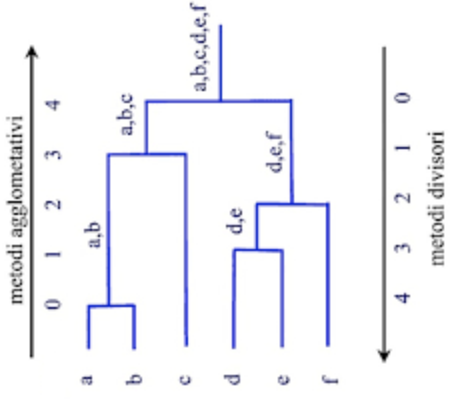
\includegraphics[width=8cm]{C_Gerarchico1.png}
\caption{Esempio di dendogramma\protect\footnotemark}
\label{fig:esempio di clustering gerarchico}
\end{figure}
\footnotetext{Presa da: \url{https://www.developersmaggioli.it/wp-content/uploads/2019/06/images.png}}

\vspace{1cm}

\begin{figure}[h] \centering
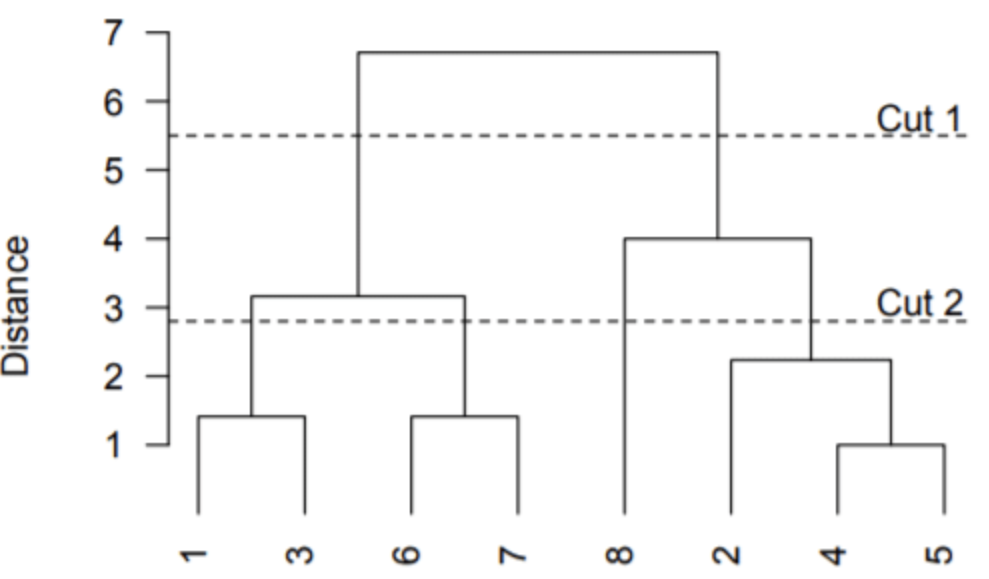
\includegraphics[width=8cm]{C_Gerarchico2.png}
\caption{Esempio di dendogramma con tagli gerarchici\protect\footnotemark}
\label{fig:esempio dendogramma}
\end{figure}
\footnotetext{Presa da: \url{https://www.researchgate.net/profile/Emanuele-Lo-Biundo/publication/344452675/figure/fig7/AS:942183599325184@1601645483382/Figura-23-Esempio-di-clustering-gerarchico-su-8-osservazioni.ppm}}

\paragraph{Clustering basato sulla densità}
Gli algoritmi di clustering basati sulla densità sono ideati per la creazione di cluster di forma arbitraria. In questo approccio, un cluster di forma arbitraria è considerato come una regione in cui la densità degli oggetti supera una soglia. Nel clustering density-based, il raggruppamento avviene analizzando l'intorno di ogni punto nello spazio. In particolare, viene considerata la densità di punti in un intorno di raggio fissato. DBSCAN e SSN RDBC sono algoritmi tipici di questo tipo.

\begin{figure}[h] \centering
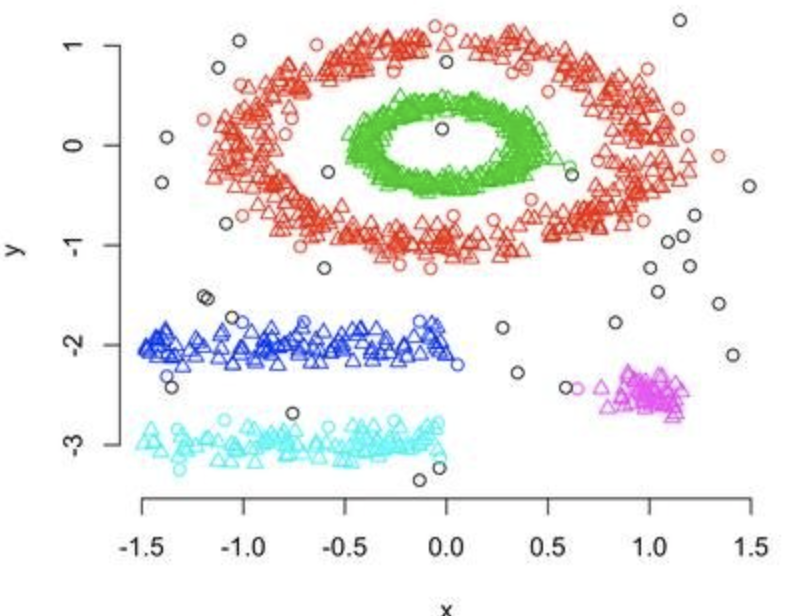
\includegraphics[width=8cm]{C_Density.png}
\caption{Esempio DBSCAN\protect\footnotemark}
\label{fig:density clustering}
\end{figure}
\footnotetext{Presa da: \url{https://www.researchgate.net/profile/Emanuele-Lo-Biundo/publication/344452675/figure/fig7/AS:942183599325184@1601645483382/Figura-23-Esempio-di-clustering-gerarchico-su-8-osservazioni.ppm}}

\vspace{2cm}
Per concludere lo schema rappresentato a figura \ref{fig:ProfilazioneML} indica che con la black-box è possibile sfruttare la capacità valutativa della board, la quale è in grado di generare uno score del guidatore e di giudicarlo in base a questo, la possibilità di classificarlo utilizzando tecniche di machine learning o la possibilità di utilizzare entrambe le tecniche per avere un quadro completo relativo al suo stile di guida.

\vspace{0.5cm}
\begin{figure}[h]
\centering
\begin{tikzpicture}[node distance=2cm]

% Definizione dei nodi
\node (ecu) [process] {ECU};
\node (obd) [process, below of=ecu] {OBD-II adapter};
\node (profiling) [process, below of=obd] {Driver profiling};
\node (score) [process, below of=profiling, xshift=-3.5cm] {Score obtained by board};
\node (ml) [process, below of=profiling, xshift=3.5cm] {Machine Learning technique};

% Connessione tra i nodi
\draw [arrow] (ecu) -- (obd);
\draw [arrow] (obd) -- (profiling);
\draw [arrow] (profiling) -- (score);
\draw [arrow] (profiling) -- (ml);

\end{tikzpicture}
\caption{Diagramma di flusso del sistema di profilazione conducente: la board è in grado di attribuire un voto al conducente, è inoltre possibile affiancare a questa capacità delle tecniche di machine learning adoperate per classificare lo stile di guida dei diversi clienti della flotta}
\label{fig:ProfilazioneML}
\end{figure}

\chapter*{Ringraziamenti}
\addcontentsline{toc}{chapter}{Ringraziamenti}  % Aggiunge i ringraziamenti all'indice
Giunto alla conclusione di questo cammino, mi rendo conto che il percorso universitario non è stato solo una crescita personale e accademica, ma anche un percorso arricchito dalla presenza di persone che hanno contribuito a rendere questa esperienza unica.
Vorrei ringraziare profondamente la mia famiglia, per il loro supporto, l'incoraggiamento costante e la fiducia che hanno sempre riposto in me; i vostri sacrifici e la vostra pazienza mi hanno dato la forza di superare ogni difficoltà e raggiungere questo importante traguardo.
Un grazie particolare va a mio fratello, che è stato un esempio di determinazione e impegno. Il suo sostegno e la sua capacità di farmi vedere il lato positivo in qualsiasi circostanza in cui ci si trova, hanno fatto la differenza in molte occasioni.
Un pensiero affettuoso va ai miei amici e colleghi, che hanno condiviso con me gioie e sfide durante questi anni. Grazie per avermi sempre ricordato l'importanza di ridere, di prendersi delle pause e di vivere ogni momento con entusiasmo.
Un ringraziamento speciale va al mio relatore, che con pazienza, disponibilità e competenza mi ha guidato in questo percorso. La sua prontezza nel rispondere a ogni mio dubbio e nel chiarire ogni mia domanda è stata fondamentale per la realizzazione di questa tesi e per la mia crescita accademica.
Infine, il mio ringraziamento più sentito va alla mia ragazza, il cui amore, la cui pazienza e la cui comprensione hanno reso possibile tutto questo. Sei stata al mio fianco in ogni passo, offrendo sempre il tuo sostegno e la tua presenza, e per questo ti sarò sempre grato.

\printbibliography[title={Bibliografia}]

\end{document}
